%\documentclass[preprint]{aastex}  % USE THIS TO MAKE BIB, THEN FORMAT USING EMULATEAPJ
\documentclass[twocolumn,apj,numberedappendix]{emulateapj}
\shorttitle{Fringe-Rate Filtering}
\shortauthors{Parsons, et al.}

\usepackage{amsmath}
\usepackage{graphicx}
\usepackage[figuresright]{rotating}
%\usepackage{rotating}
\usepackage{natbib}
%\usepackage{pdflscape}
%\usepackage{lscape}
\citestyle{aa}

\def\b{\mathbf{b}}
\def\k{\mathbf{k}}
\def\r{\mathbf{r}}
\def\q{\mathbf{q}}
\def\b{\mathbf{b}}
\def\kp{\mathbf{k}^\prime}
\def\kpp{\mathbf{k}^{\prime\prime}}
\def\V{\mathbb{V}}
\def\At{\tilde{A}}
\def\Vt{\tilde{V}}
\def\Tt{\tilde{T}}
\def\tb{\langle T_b\rangle}
\newcommand{\vis}{\mathbf{v}}
\newcommand{\x}{\mathbf{x}}
\newcommand{\xhat}{\hat{\mathbf{x}}}
\newcommand{\A}{\mathbf{A}}
\newcommand{\N}{\mathbf{N}}
\newcommand{\rhat}{\hat{\mathbf{r}}}

\begin{document}
\title{Fringe-Rate Filtering}

\author{
Aaron R. Parsons\altaffilmark{1,2},
Adrian Liu\altaffilmark{1},
%James E. Aguirre\altaffilmark{3},
%Zaki S. Ali\altaffilmark{1},
%David R. DeBoer\altaffilmark{2},
%Daniel C. Jacobs\altaffilmark{8},
%David F. Moore\altaffilmark{3},
%Jonathan C. Pober\altaffilmark{1},
% XXX if includes paper data, needs full author list
}

\altaffiltext{1}{Astronomy Dept., U. California, Berkeley, CA}
\altaffiltext{2}{Radio Astronomy Lab., U. California, Berkeley, CA}
\altaffiltext{3}{Dept. of Physics and Astronomy, U. Pennsylvania, Philadelphia, PA}
\altaffiltext{8}{School of Earth and Space Exploration, Arizona State U., Tempe, AZ}

\begin{abstract}
\end{abstract}

% XXX fringe weighting profile
% XXX delay spectrum not violated by freq-dependent fringe rate weights




\section{Introduction}

[XXX: Rework intro to make connection to 21cm more explicit.]

In any observation of the sky, integrating in time results in increased sensitivity.  Such increased sensitivity is particularly important in applications where instrumental noise levels are expected to be high compared to the faint signals that one seeks to measure.  As an example of this, in recent years multiple instruments have been built in an attempt to detect the redshifted $21\,\textrm{cm}$ line from the Epoch of Reionization\footnote{In this paper, we will frequently use $21\,\textrm{cm}$ interferometric arrays as example instruments with which to focus our discussion, and indeed, Sections XXX pertain only to such arrays.  However, we emphasize that the central idea of this paper---that fringe-rate filtering can be used to combine time-ordered data in a way that maximizes sensitivity---is one that should be widely applicable to any interferometer.}.  At the relevant redshifts ($z\sim 6$ to $20$), theoretical models suggest that this cosmological signal will be faint, on the order of $1\,\textrm{mK}$ in brightness temperature, while a typical instrument's system temperature is typically $\sim 100\,\textrm{K}$.  Long time-integrations are therefore crucial, and as a practical matter, this is often accomplished by accumulating time-samples, either in the image domain or in Fourier space.  In both cases, one is essentially making maps, which can be shown to be in principle a lossless method of data compression, and therefore an attractive method for realizing the increased sensitivity that time-integration provides.

The quest for increased sensitivity, however, has often led to instrumental designs that have made mapmaking algorithms rather unwieldy.  Consider first the possibility of accumulating time-samples in the image domain, again for the special case of a $21\,\textrm{cm}$ interferometer array.  To increase sensitivity, such arrays typically have wide fields-of-view and are configured to yield a large number of redundant baselines.  Over long time-integrations, imaging wide fields-of-view requires careful attention to curved-sky artifacts, which can become computationally expensive to control, particularly if the pixelization is taken to be extremely fine to avoid artifacts from gridding.  While a fine pixelization is necessary for mapmaking to be lossless (XXX: cite], this can become wasteful for interferometers with a large number of redundant baselines, in the sense that a large number of pixels are needed to store information about a small number of Fourier modes. [XXX: Make the connection in this last sentence a little clearer.]

Mapmaking in Fourier space (or more precisely, on the $uv$-plane) alleviates some of these problems.  Fourier space is a natural space for the accumulation of interferometric data, for there each baseline probes a relatively localized region.  It is therefore a particularly economical basis for accumulating interferometric data, especially if the final goal is to produce a spatial power spectrum, or other quantities that are ``native" to Fourier space.  However, gridding artifacts remain, and are even more troublesome when power spectrum estimation is considered in the context of rotation synthesis.  As the Earth rotates, baselines sample a series of points along tracks on the $uv$-plane.  Nearby points are almost perfectly correlated, and ought to be integrated coherently prior to the squaring step of any power spectrum measurement, while faraway points can only be combined statistically after squaring.  Unless one is willing to keep track of the level of correlation of every $uv$-point with every other $uv$-point, an arbitrary choice must be made as to how far away from each other two points can lie before they are considered incoherent.  Often, this choice is encapsulated by the $uv$-pixel size (particularly in calculations of power spectrum sensitivity XXX: cite), with samples falling in the same cells labeled as coherent, and those in different cells labeled as incoherent.  However, this can potentially lead to a loss of sensitivity in combining samples that straddle pixel boundaries.  While these obstacles can in principle be overcome, it is clear that extreme care must be taken in the mapmaking process to ensure that the full sensitivity of an interferometer array is realized.

In this paper, we introduce a new method for combining time-ordered data---fringe-rate filtering---that avoids the aforementioned pitfalls while affording one the advantages traditionally reserved only when mapmaking.  The essential idea is that for an interferometer operating in a drift-scan observing mode, celestial sources of emission have predictable fringe-rates 

\begin{itemize}
\item For any instrument, important to integrate in time.  This is how you get sensitivity.
\item Historically (and what is conceptually the easiest) is to make a map and to bin there.
\item However, mapmaking is i) difficult, especially with the widefield instruments, ii) subject to artifacts and systematics such as gridding artifacts, iii) ``wasteful" for an interferometer array with high redundancy, since the image basis is not efficient if you're only measuring a small number of modes, iv) unnecessary if you're using an interferometer to measure a power spectrum.
\item For interferometers trying to measure a power spectrum, it'd be nice to be able to stay in the natural ``Fourier" space defined by an interferometer.
\item On the other hand, there are advantages to mapmaking that we want: i) coherent integrations in time, ii) the mitigation of systematics (such as polarization leakage), iii) the ability to down-weight data towards the edge of the primary beam (the instrument has already done that once, but an optimal inverse-variance weighted estimator needs to do it once again).  Not clear how to do that if one doesn't go to the image-domain.
\item In this paper, we introduce a method---fringe-rate filtering---that allows one to stay in visibility space but still get all the advantages of mapmaking.  The paper is geared towards drift-scan telescopes, although some of the lessons are also applicable to tracking telescopes.  The central idea is to Fourier-transform the time-series in order to sort the observations by fringe-rate, and then to enact a low-pass filter.  Since different parts of the sky have different interferometer fringe-rates, a careful tailoring of the filter can downweight different parts of the sky, allowing one to perform the downweightings towards the edge of the primary beam.
\item Fringe-rate space is particularly good for identifying high versus low signal-to-noise modes, because certain fringe-modes are physically impossible for true celestial emission (mention the super high azimuthal mode caveat here).  We can eliminate those modes.  This also makes it clear that time-averaging visibilities is not good.  Because it's a sinc in fringe-rate space, which has some high fringe-rate components.

\item Fringe-rate filters can be optimized to maximize sensitivity, assuming a noise power spectrum.  But they can also be used to help fight systematics.  As an example, 21cm arrays suffer from polarization leakage.  This can be particularly hard to fight because of the redundancy in the arrays.  Beam-sculpting, though, helps reduce this.  Specific to 21cm arrays, also show that we don't mess up delay-spectrum.
\item Other similar things in literature.  Richard's $m$-mode formalism made more explicit.  Optimal mapmaking.  Delay/DDR paper.  Also look at Andre's stuff.
\item Outline the paper.
\end{itemize}
Further details are supplied in Appendices A and B of \citet{parsons_et_al2013}.

\begin{equation}
\tilde{V}(\tau)=\int{W(\nu)\cdot S(\nu)\cdot V(\nu)e^{-2\pi i\nu\tau}~d\nu},
\label{eq:dtransform}
\end{equation}


\section{Combining time-ordered data in an optimal way for mapmaking}

[XXX: Say somewhere that unless otherwise stated, considering a drift-scan telescope.]
[XXX: Don't forget to define hats as estimators, once and for all.]
In this section, our goal is to examine how time-ordered visibilities from an
interferometer should be best combined into information about the sky (such as
an image-domain map).  Contrary to expectations, we will find that it is
suboptimal to pursue the traditional, straightforward approach of averaging
data in time, in the sense that such a procedure gives rise to
larger-than-necessary error bars.  Instead, employing an unbiased,
minimum-variance prescription naturally yields the technique of
\emph{fringe-rate filtering}, the subject of this paper.

Suppose our time-ordered visibilities are grouped into a measurement vector
$\vis$ of length $N_b N_t$, where $N_b$ is the number of baselines, and $N_t$
is the number of snapshots taken in time.  If we represent the true sky as a
vector $\x$ of length $N_\textrm{pix}$, and our instrument's response as a
matrix $\A$ of size $N_b N_t \times N_\textrm{pix}$, the measurement equation
is given by
\begin{equation}
\label{measEqn}
\vis = \A \x + \mathbf{n},
\end{equation}
where $\mathbf{n}$ is a noise vector.  Note that in this general form, Equation
\eqref{measEqn} is not basis-specific.  For example, while it is often useful
to think of $\x$ as a vector containing a list of temperatures in a set of
pixels on the sky (hence the variable name $N_\textrm{pix}$), it is equally
valid to employ another basis, such as spherical harmonics.  Similarly, while
we call $\vis$ the time-ordered data, it need not be a time series, and in
fact, a central message of this paper is that an optimal data analysis
prescription is more naturally phrased in terms of the Fourier dual to time,
i.e. fringe-rate.

Given our measurement $\vis$, the optimal estimator $\xhat$ of the true sky
$\x$ is given by \citep{Tegmark97,Morales2009}
\begin{equation}
\label{optEst}
\xhat = \left[ \A^\dagger \N^{-1} \A \right]^{-1} \A^\dagger \N^{-1} \vis,
\end{equation}
where $\N$ is the noise covariance matrix, defined as $\langle \mathbf{n}
\mathbf{n}^\dagger \rangle$, with angled brackets denoting an ensemble average.
Again, our vector/matrix expressions are basis-independent, so even though the
formation of $\xhat$ is often described as ``mapmaking", it need not correspond
to spatial imaging in the traditional sense.  Regardless of the basis we work
in, this estimator is unbiased, i.e.
\begin{equation}
\label{unbiased}
\langle \xhat \rangle = \x,
\end{equation}
and has minimum variance, which is given by
\begin{equation}
\label{eq:sigma}
\boldsymbol \Sigma \equiv \langle (\x - \xhat) ( \x - \xhat)^\dagger \rangle = \left[ \A^\dagger \N^{-1} \A \right]^{-1}.
\end{equation}
The estimator given by Equation \eqref{optEst} can also be proved to be
lossless \citep{Tegmark97}, in the sense that any quantities (such as power
spectra) formed further downstream in one's analysis will have identically
small error bars whether one forms these data products from $\xhat$ or chooses
to work with the larger and more cumbersome set of original data $\vis$.

[XXX: add that the unbiased condition holds only when the matrix is invertible.]

In principle, Equation \eqref{optEst} is all that is needed to optimally
estimate the true sky.  One simply forms the relevant matrices and performs the
requisite matrix inversions and multiplications.  However, this is
computationally infeasible in practice, given that modern-day interferometers
are comprised of a large number of baselines operating over long integration
times, resulting in rather large matrices.  This is what motivated the authors
of \cite{Shaw2013} to propose their $m$-mode formalism, essentially rendering
many of the relevant matrices sparse, making them computationally easy to
manipulate.  While the $m$-mode formalism is a general framework that can be
used to solve a variety of problems (such as mitigating foreground
contamination), our goal here is to develop similarly convenient techniques for
the mapmaking problem (i.e., the formation of $\xhat$), with much detail
devoted to the intuition behind how our optimal estimator operates for an
interferometer.

\subsection{The general sub-optimality of time integration}
\label{timeSubOpt}

We begin by showing that it is suboptimal to make maps by integrating in time.
Consider the visibility response $V_b(t)$  of an interferometer baseline $b$ at
time $t$ to the sky $T(\rhat)$:
\begin{eqnarray}
\label{generalVis}
V_b(t) &&= \int B(\rhat, t) T(\rhat) \exp \left[ -i 2 \pi \left( \frac{b_y}{\lambda} \cos \eta \cos \theta \right) \right] \nonumber \\
&& \times  \exp \left[ -i 2 \pi \left( \frac{b_0}{\lambda} \sin \theta \sin(\varphi - \omega_\Earth t ) \right) \right]  d\Omega +n(t), \qquad
\end{eqnarray}
where $n(t)$ is the instrumental noise, $\theta$ and $\varphi$ are polar and
azimuthal angles fixed to the celestial sphere, respectively, $B(\rhat,t)$ is
the primary beam, $\lambda$ is the wavelength, $\omega_\Earth$ is the angular
frequency of the Earth's rotation, $\eta$ is the geographic latitude of the
array, and $b_0 \equiv \sqrt{b_x^2 + b_y^2 \sin^2 \eta}$, where $b_x$ and $b_y$
are the east-west and north-south baseline lengths, respectively.  With this
measurement equation, we are assuming that the primary beam is fixed with
respect to local coordinates and translates azimuthally on the celestial
sphere.  We additionally assume that the baseline is phased to zenith.  In
other words, Equation \eqref{generalVis} describes an interferometer observing
in a drift-scan mode.

To see how integrating in time may be suboptimal, consider a simplified, purely
pedagogical thought experiment where our interferometer consists of a single
east-west baseline ($b_y=0$) situated at the equator ($\eta = 0$).  For the
primary beam, suppose we have a beam that is extremely narrow in the polar
direction, so that $B(\rhat, t) \equiv \delta(\theta - \pi / 2)
B_\varphi(\varphi-\omega_\Earth t)$.  Plugging these into restrictions into our
equation, we obtain
\begin{eqnarray}
\label{simpVis}
V_b (t) && = \int  \, B_\varphi(\varphi-\omega_\Earth t)  T \left( \theta = \frac{\pi}{2}, \varphi \right) \nonumber \\
&&\times \exp \left[ -i 2 \pi  \frac{b_x}{\lambda} \sin(\varphi - \omega_\Earth t ) \right] d\varphi+ n(t).
\end{eqnarray}
Now suppose we have a large number of different baselines, so that we have
multiple copies of this equation, representing a time series for each baseline.
Grouping these time series into a vector gives the continuous version of
$\vis$.  We can similarly identify $n(t)$ and $T(\theta= \pi / 2, \varphi)$ as
the continuous versions of $\mathbf{n}$ and $\x$ respectively, with the rest of
the Equation \eqref{simpVis}'s integrand as the continuous version of $\A$.  We
can model the noise covariance between baselines $b$ and $b^\prime$, at times
$t$ and $t^\prime$ as
\begin{equation}
\label{eq:noiseCovar}
N_{bb^\prime} (t, t^\prime) = \sigma^2 \delta_{bb^\prime} \delta(t-t^\prime),
\end{equation}
where $\sigma$ is an root-mean-square noise level assumed to be uncorrelated in
time and uncorrelated between baselines.

To see how the optimal prescription of Equation \eqref{optEst} combines
information from different times, we need only evaluate $\A^\dagger \N^{-1}
\vis$, for the subsequent application of $\left[ \A^\dagger \N^{-1} \A
\right]^{-1}$ only serves to undo the effects of an instrument's synthesized
beam once the time series have already been combined.  In our toy model, we
have
\begin{equation}
\label{toyComb}
\left( \A^\dagger \N^{-1} \vis \right)_{\varphi} \! = \! \sum_b \!\!  \int \frac{dt}{\sigma^2} \,  B_\varphi(\varphi-\omega_\Earth t) \, e^{ i 2 \pi  \frac{b_x}{\lambda} \sin(\varphi - \omega_\Earth t ) } V_b(t),
\end{equation}
where the $\varphi$ variable serves as the continuous version of a discrete
vector index.  This expression shows that the optimal, minimum variance
prescription does not call for the integration of visibilities in time.
Instead, our expression calls for the \emph{convolution} of the visibility data
with a kernel that is specified by the primary beam shape and the baseline.

Now, recall from the convolution theorem that convolution in time is equivalent
to multiplication in the Fourier dual space of time.  For an interferometer
baseline, this Fourier dual space is fringe-rate.  Equation \eqref{toyComb}
therefore suggests that the optimal way to combine different time samples is to
express visibilities in fringe-rate space, and then to weight different
fringe-rates appropriately before summing.  We will develop this type of
fringe-rate filtering in full generality in Section \ref{fringeRateIntro},
demonstrating that its optimality is not a peculiarity of our current
pedagogical example, but is instead applicable in all situations.

%It is also important to emphasize that the technique of instantaneous
%snapshots---where one uses information from different baselines to form an
%instantaneous snapshot of the sky, which is then averaged with other snapshots
%to form a final image---is also sub-optimal.  In our notation, this would
%correspond to 

\subsection{The special case where integrating in time is optimal}

Before proceeding, it is instructive to establish the special case where time
integration is the optimal technique, since it is used so ubiquitously in the
literature.  An inspection of Equation \eqref{toyComb} shows that were it not
for the time-dependence in the primary beam and the time-dependence of the sky
moving through a baseline's fringes, the optimal recipe would indeed reduce to
an integration of visibilities in time.  Finding the limit where time
integration is optimal is then equivalent to finding a special case where the
aforementioned time-dependences vanish.

Recall that in our previous example, the primary beam had a time-dependence
only because our thought-experiment consisted of a drift-scan telescope, whose
measurement equation was written in coordinates fixed to the celestial sphere.
Instead of this, suppose one had a narrow primary beam that tracked a small
patch of the sky.  The primary beam would then have a fixed shape in celestial
coordinates, and $B(\rhat, t)$ would simply become $B(\rhat)$ in Equation
\eqref{generalVis}.  To attempt to nullify the time-dependence of fringes
sweeping across the celestial sphere, one may phase the visibilities in a
time-dependent way, essentially tracking the center of the patch as it moves
across the sky.  Putting this all together and assuming that the primary beam
is narrow enough to justify a flat-sky approximation, the measurement equation
becomes
\begin{eqnarray}
\label{flatSkyVis}
V_b(t) &&= \int B(\rhat) T(\rhat) \exp \left[ -i 2 \pi \left( \frac{b_0}{\lambda}  \sin(\varphi - \omega_\Earth t )\right) \right] \nonumber\\
&&\!\!\! \times \exp \left[-i 2 \pi \left( \frac{b_y}{\lambda} \cos \eta \sin \theta \right) + i \psi(t) \right] d\Omega +n(t), \qquad
\end{eqnarray}
where we have assumed for simplicity that the center of our small field is
directly above the equator, and that a time-dependent phase $\psi(t)$ has been
applied.  With this, the optimal combination of time-ordered data becomes
\begin{eqnarray}
\left( \A^\dagger \N^{-1} \vis \right)_{(\theta,\varphi)}^\textrm{flat} &&  = \frac{B(\theta, \varphi)}{\sigma^2} e^{i 2 \pi \frac{b_y}{\lambda} \cos \eta \sin \theta}  \nonumber  \\
&&\!\!\! \times \sum_b \int  dt \,\,e^{ i 2 \pi  \frac{b_x}{\lambda} \sin(\varphi - \omega_\Earth t ) -i \psi (t) } V_b(t). \qquad
\end{eqnarray}
This is still not quite a simple average in time because there is no choice of
$\psi(t)$ that can cancel out the time-dependence of $\sin (\varphi -
\omega_\Earth t)$ for all $\varphi$ and all $t$.  Another way to phrase the
problem is to note that even in the flat-sky approximation, one cannot expand
Taylor expand $\sin (\varphi - \omega_\Earth t)$ over long observation times.
With short observations, however, an expansion is justified, and picking
$\psi(t) = 2 \pi \frac{b_x}{\lambda} \omega_\Earth t$ gives
\begin{eqnarray}
\left( \A^\dagger \N^{-1} \vis \right)_{(\theta,\varphi)}^\textrm{flat,short} =  &&\frac{B(\theta, \varphi)}{\sigma^2} e^{i 2 \pi \left( \frac{b_y}{\lambda} \cos \eta \sin \theta + \frac{b_x}{\lambda} \sin\varphi \right)} \nonumber \\
&& \times \sum_b   \int  dt \, V_b(t),
\end{eqnarray}
which is a simple averaging in time.  In short, then, integrating in time is an
optimal way to combine time-ordered data only if a number of criteria are met:
the flat-sky approximation must hold, the primary beam must track the field,
the visibilities must be phased to track the center of the field, and the
observations must be short.

[XXX: talk about how the same issues apply for a $uv$-plane description.]

[XXX: Maybe mention instantaneous snapshots and how it relates?]

[XXX: Fringe stopping at higher frequencies.]

\subsection{Fringe-rate filtering}
\label{fringeRateIntro}

We now proceed to derive the optimal prescription for combining time-ordered
data, which will lead us to the technique of fringe-rate filtering.  Because
our derivation will \emph{not} require any of the approximations that we have
invoked so far for pedagogical reasons, we will begin with our general
expression for time-ordered visibilities, Equation \eqref{generalVis}.  From
our toy example [Equation \eqref{toyComb}], we know that fringe-rate space (the
Fourier dual of time) is a promising space in which to combine time-ordered
data.  Formally, measurements in this space are given by
\begin{equation}
\widetilde{V}_b (f) \equiv \frac{1}{T_\Earth} \int_{-T_\Earth / 2}^{T_\Earth /2} dt \exp \left( - 2 \pi i f t \right) V_b (t),
\end{equation}
where $f$ is the fringe-rate, and $T_\Earth = 2 \pi / \omega_\Earth$ is the
Earth's rotation period.  It is natural to work in fringe-rate bins such that
the $n^{th}$ bin is given by $f_n \equiv n / T_\Earth$, where $n$ is an
integer.  The measurement in the $n^{th}$ bin is then given by
\begin{eqnarray}
\label{fringeVis}
\widetilde{V}_b (f_n) &&= \int d\Omega \, T(\rhat) e^{-i 2 \pi  \frac{b_y}{\lambda} \cos \eta \cos \theta} \nonumber \\
&& \!\!\!\times  \int_{-\frac{T_\Earth}{ 2}}^{\frac{T_\Earth}{2}} \frac{dt}{T_\Earth} \, B(\rhat, t) e^{ -i  \frac{2 \pi n t}{T_\Earth} +i  \frac{2\pi b_0}{\lambda} \sin \theta \sin \left( \omega_\Earth t - \varphi \right)}, \qquad
\end{eqnarray}
where we have temporarily omitted the additive noise term to avoid mathematical
clutter.  To proceed, we make some simplifying assumptions (although only some
of which are absolutely required).  First, assume that we are once again
considering a drift-scan instrument.  If the primary beam shape is
approximately separable, we can then say
\begin{equation}
B(\rhat, t) \equiv B_\theta (\theta) B_\varphi (\varphi - \omega_\Earth t),
\end{equation}
where $B_\varphi$ is a function with period $2\pi$.  Taking advantage of this periodicity, we can write the beam as
\begin{equation}
B(\rhat, t) = B_\theta (\theta) \sum_q \widetilde{B}_q e^{-iq \varphi} e^{i q \omega_\Earth t},
\end{equation}
where $\widetilde{B}_q \equiv \int \frac{d\varphi}{2\pi} B_\varphi(\varphi)
e^{i q\varphi}$ is the $q^{th}$ Fourier coefficient.  Plugging this into
Equation \eqref{fringeVis} and making the substitution $\psi \equiv
\omega_\Earth t - \varphi$, one obtains
\begin{eqnarray}
\widetilde{V}_b (f_n) &&= \int d\Omega \, T(\rhat) B_\theta (\theta) e^{-i 2 \pi  \frac{b_y}{\lambda} \cos \eta \cos \theta} \nonumber \\
&& \times \sum_q \frac{\widetilde{B}_q e^{-i n \varphi}}{2 \pi} \int_{-\pi -\varphi}^{\pi+\varphi} d\psi \, e^{i (q-n) \psi +i \frac{2 \pi b_0}{\lambda} \sin \theta \sin \psi}. \qquad
\end{eqnarray}
Now, note that the integral over $\psi$ is of a periodic function over one
period.  We may therefore freely shift the limits of the integral by a constant
amount without affecting the result.  In particular, we may remove the
$+\varphi$ terms in the limits (the only restriction being that having performed a $\varphi$-dependent shift, it is no longer legal to permute the various integrals), and
the result is a standard integral form for a Bessel function $J$ of the first
kind:
\begin{eqnarray}
\label{fringeBessel}
\widetilde{V}_b (f_n) =&& \int \frac{d\Omega}{2 \pi}\, T(\rhat) B_\theta (\theta) e^{-i 2 \pi  \frac{b_y}{\lambda} \cos \eta \cos \theta}
e^{-i n \varphi} \nonumber \\ 
&& \times \sum_q \widetilde{B}_q  J_{n-q} \left( \frac{2 \pi b_0}{\lambda} \sin \theta \right).
\end{eqnarray}
Several features are of note here.  For wide primary beams, $\widetilde{B}_q$
is sharply peaked around $q=0$, so the terms following the sum over $q$
essentially amount to $J_n ( 2 \pi b_0 \sin \theta / \lambda )$.  Now, notice
that the argument of the Bessel function is bounded, always lying between $\pm
2\pi b_0/ \lambda$.  For large $n$ (high fringe-rate bins), then, one can use
the small argument asymptotic form for $J_n$,\begin{equation}
J_n \left( \frac{2 \pi b_0 \sin \theta}{ \lambda} \right) \approx \frac{1}{n!} \left( \frac{ \pi b_0 \sin \theta}{ \lambda} \right)^n,
\end{equation}
which is a sharply decreasing function of $n$ for large $n$.  This means that
there must be very little sky signal at high fringe-rate bins.  Intuitively,
this is because sources on the celestial sphere have their fringe rates limited
by the Earth's rotation period and projected baseline length $b_0$, making high
fringe rates physically unattainable by true celestial emission.  Any signals
seen in high fringe-rate bins will therefore be primarily due to noise.

With celestial emission appearing only in low fringe-rate bins, it is
reasonable to expect that one can reduce noise (in other words, achieving the
goals of time integration) by Fourier transforming the data into fringe-rate
space and downweighting (or discarding) high fringe-rate modes.  This is
confirmed by constructing the optimal prescription as we did above, which
yields
\begin{eqnarray}
\label{eq:AdagNinvv}
\left( \A^\dagger \N^{-1} \vis \right)_{\theta,\varphi} && = \frac{B_\theta^* (\theta)  \sin \theta}{2\pi \sigma^2} \sum_{b,n} e^{i n \varphi} e^{i 2 \pi  \frac{b_y}{\lambda} \cos \eta \cos \theta} \nonumber \\
&& \times \sum_{q} \widetilde{B}_q^* J_{n-q} \left( \frac{2 \pi b_0}{\lambda} \sin \theta \right) \widetilde{V}_b (f_n).
\end{eqnarray}
In words, this recipe instructs us to move into fringe-rate space (where the
sky emission is already concentrated in $f_n$) and to further downweight by
$\sum_{q} \widetilde{B}_q^* J_{n-q} \left( \frac{2 \pi b_0}{\lambda} \sin
\theta \right)$, which, as we have argued above, is small for high fringe
rates.  Thus, low-pass fringe-rate filtering is the optimal way to combine
time-ordered data from an interferometer.

[XXX: Talk about how we're only going to use these to guide intuition, and more numerical stuff later in the paper.]

\subsection{The possibility of deconvolution}

%Unlike the narrow-beam toy example of Section \ref{timeSubOpt}, Equation
%\eqref{fringeBessel} reveals that in general, the fringe-rate response of a
%celestial source depends on the declination of the source.  Sources near the
%celestial pole tend to have low fringe rates, whereas those near the celestial
%equator tend to have higher fringe rates, as one can see in Figure [XXX: insert
%figure refrence].  Applying a filter in fringe-rate space therefore
%geometrically selects certain parts of the sky, effectively narrowing the
%primary beam of the observation.  To see this, consider an interferometer
%baseline of length $16 \lambda$, located at the equator.  Neglecting the
%effects of the instrument's primary beam, the contribution of sources to
%$\widetilde{V}_b (f_n)$ at various $\theta$ is given by $ J_n ( 2 \pi b_0 \sin
%\theta / \lambda ) \sin \theta$.  This function has a broad response over a
%large range of $\theta$, as one can see in the left column of Figure
%\ref{besselContributions}.  However, this response is highly oscillatory away
%from zero declination ($\theta = \pi/2$) and therefore cancels out near
%celestial poles, particularly for low fringe-rate bins.  To quantify this, we
%plot in the right panels of Figure \ref{besselContributions} the cumulative
%effect of sources at various $\theta$, i.e.
%\begin{equation}
%\label{eq:cumulResponse}
%I_n ( \theta) \equiv \int_0^\theta J_n \left( \frac{2 \pi b_0 \sin \gamma }{ \lambda} \right) \sin \gamma \, d\gamma,
%\end{equation}
%and ask which range of $\theta$ values contribute most to the final result
%$\widetilde{V}_b (f_n) \propto I_n (\pi /2)$.  One sees that for the low
%($n=5$) fringe-rate bin, most of the contribution to $\widetilde{V}_b (f_n)$
%comes from a narrow region around $\theta \approx \pi / 2$, whereas for the
%higher fringe-rate, a broader range of declinations contribute to the final
%result.  A fringe-rate filter that downweights high fringe-rates therefore
%narrows the effective beam.
%
%We now compute more rigorously quantify the notion of an effective beam.  Note
%that 
If one has a sufficient number of baselines (roughly speaking, a
``fully-filled $uv$-plane"), then the application of $ \left[ \A^\dagger
\N^{-1} \A \right]^{-1}$ should perfectly deconvolve instrumental beams in our
estimator of the sky [Equation \eqref{optEst}] and leave a delta-function
effective beam.  Indeed, this is precisely what Equation \eqref{unbiased}
states.  However, in practice the matrix $\A^\dagger \N^{-1} \A$ may not be
invertible, and the best that one can do is to produce an estimate that is
convolved (or only partially deconvolved) with an effective beam.

The question of whether one has a sufficient density of baselines to deconvolve
out the beam is most easily answered by writing $\A$ and $\A^\dagger \N^{-1}
\A$ in convenient bases.  We first rewrite Equation \eqref{fringeBessel} so
that it expresses a given baseline's fringe-rate measurements in terms of
azimuthal Fourier modes $a_m(\theta)$ of the sky $T(\theta, \varphi) = \sum_m
a_m(\theta) e^{i m \varphi}$.  The measurement equation becomes
\begin{eqnarray}
\label{eq:convenientBasis}
\widetilde{V}_b (f_n) && = \sum_m \int d\theta \, B_\theta (\theta) \sin \theta  \, e^{-i 2 \pi  \frac{b_y}{\lambda} \cos \eta \cos \theta} \nonumber \\
&& \times \sum_q \widetilde{B}_q  J_{n-q} \left( \frac{2 \pi b_0}{\lambda} \sin \theta \right) \delta_{mn} a_m (\theta).
\end{eqnarray}
The Kronecker delta function appears because for a drift-scan telescope, the
time coordinate uniformly maps to the azimuthal angle $\varphi$ (or
equivalently, the Fourier index $m$ uniformly maps to fringe-rate bin), as
emphasized in \cite{Shaw2013}.  From the expression we can immediately read off
the form of $\A$ in this basis, and inserting it into $\A^\dagger \N^{-1} \A$
results in
\begin{equation}
\label{manifest}
\left( \A^\dagger \N^{-1} \A \right)_{m, \theta ; m^\prime \theta^\prime} = \frac{\delta_{m m^\prime}}{\sigma^2} \sum_b \lambda_b^m \, h_b(\theta, m) \, h_{b}^*(\theta^\prime, m^\prime),
\end{equation}
where we have once again taken $\N$ to be diagonal, with entries $\sigma^2$, and have made the definitions
\begin{eqnarray}
&& g_b(\theta, m) \equiv B_\theta^*(\theta) \sin \theta \exp \left(i 2 \pi  \frac{b_y}{\lambda} \cos \eta \cos \theta\right) \nonumber \\
&& \qquad \qquad \quad \times \sum_q \widetilde{B}^*_q  J_{m-q} \left( \frac{2 \pi b_0}{\lambda} \sin \theta \right) \\
&&  h_b ( \theta, m) \equiv \frac{g_b (\theta, m)}{\sqrt{\lambda_b^m}} \\
&& \lambda_b^m \equiv  \int_0^\pi |g_b (\theta, m) |^2 d\theta .
\end{eqnarray}

Whether or not $\A^\dagger \N^{-1} \A$ is invertible for a given baseline
distribution is manifestly clear from the form of Equation \eqref{manifest}.
Imagining $\A^\dagger \N^{-1} \A$ as a discrete matrix with each side cycling
through polar angle $\theta$ more rapidly than azimuthal Fourier mode number
$m$, we see that our matrix is block diagonal.  Invertibility then hinges on
satisfying two requirements.  First, none of the blocks can be identically
zero.  While in principle this can never happen, in practice this will be the
case for sufficiently high $m$, since $m$ can be thought of as a fringe-rate
bin index, and very high fringe-rates are physically unattainable unless one
has very long baselines.  Put another way, the arguments in the previous
section for a high fringe-rate cutoff ensure that $\lambda_b^m$ gets very small
for large $m$.  For invertibility, then, one needs to either have a cutoff in
$m$ (which then defines a resolution scale in the $\varphi$ direction), or
sufficiently long baselines.

The second requirement for invertibility comes from the fact that a block
diagonal matrix's inverse is again block diagonal, with each block replaced by
its inverse.  We therefore require the invertibility of each block, which is
obtained by setting $m=m^\prime$ in Equation \eqref{manifest}, and is indexed
by $(\theta, \theta^\prime)$.  Now, notice that were we to discretize our
expression, it would have precisely the form of an eigenvalue decomposition
$\sum_i \lambda_i \mathbf{w}_i \mathbf{w}_i^\dagger$ of an arbitrary matrix,
where $\lambda_i$ is the matrix's $i^{th}$ eigenvalue and $\mathbf{w}_i$ is the
$i^{th}$ eigenvector (satisfying the normalization condition
$\mathbf{w}_i^\dagger \cdot \mathbf{w}_i = 1$).  To ensure invertibility, the
number of eigenvectors must equal the side length of the matrix.  For us, this
requirement corresponds to having the number of unique baselines be equal to or
greater than the number of angular resolution elements in the $\theta$
direction.  Intuitively, the same declinations map to different fringe-rates
for different baselines, and thus with enough baselines, one is able to take
the appropriate linear combination of different baselines to select a specific
declination and nothing else.  Importantly, this is conceptually separate from
having a variety of baseline lengths in the north-south direction and
performing synthesis imaging in the declination direction.  An examination of
the relevant expressions shows that our argument holds even if all baselines
are of a purely east-west orientation; the ability to localize in $\theta$ can
be acquired by combining fringe rates appropriately.

Having derived an expression for $\A^\dagger \N^{-1} \A$, we can also compute
the error covariance $\boldsymbol \Sigma$ of our maps.  If we have enough
baselines for invertibility, Equation \eqref{eq:sigma} says that
\begin{eqnarray}
\boldsymbol \Sigma_{m, \theta ; m^\prime \theta^\prime} &=& \left[ \A^\dagger \N^{-1} \A \right]^{-1}_{m, \theta ; m^\prime \theta^\prime} \nonumber \\
&=&  \sigma^2 \delta_{m m^\prime} \sum_b \frac{1}{\lambda_b^m} \, h_b(\theta, m) \, h_{b}^*(\theta^\prime, m^\prime).
\end{eqnarray} 
As expected, azimuthal modes corresponding to low fringe-rate bins can be
measured with high signal-to-noise.
%
%In the event of non-invertibility, on the other hand, one may elect to forgo
%the deconvolution step, and to simply normalize the estimator of the sky
%appropriately.  Put another way, as an alternative to Equation \eqref{optEst},
%we can instead use
%\begin{equation}
%\hat{\x} = \mathbf{M} \A^t \N^{-1} \vis
%\end{equation}
%as our estimator, where $\mathbf{M}$ is a diagonal normalization matrix.
%Inserting Equation \eqref{measEqn} into this and taking the ensemble average
%gives
%\begin{equation}
%\langle \hat{\x} \rangle = \mathbf{M} \A^t \N^{-1} \A \x \equiv \mathbf{B}^\textrm{eff} \x,
%\end{equation}
%where we have assumed that the instrumental noise is unbiased, so that $\langle
%\mathbf{n} \rangle = 0$, and have defined an effective beam matrix
%$\mathbf{B}^\textrm{eff}$ that is proportional to $\A^\dagger \N^{-1} \A$,
%which we have already computed in an $(m, \theta)$ basis.  If we were to
%re-express our result in a $(\varphi, \theta)$ (i.e., image) basis, each row of
%$\mathbf{B}^\textrm{eff}$ would give the weighted average of the true sky that
%forms the estimator of the sky temperature in some direction---precisely what
%one would define as an effective beam.  To ensure that these beams and our
%estimator are properly normalized, we require that each row sums to unity,
%which implicitly defines $\mathbf{M}$.  Importantly, our definition of the
%effective beam includes both the effects of the primary beam and the
%synthesized beam.
%
%For intuition and simplicity, however, suppose we stay in the $(m, \theta)$
%basis and keep $m$ fixed while we examine the behavior of the effective beam as
%a function of $\theta$ for a pure east-west baseline.  Ignoring irrelevant
%normalization constants, the result from Equation \eqref{manifest} is
%\begin{equation}
%B^\textrm{eff} (\theta) \propto B_\theta (\theta) \sin \theta \sum_q \widetilde{B}_q  J_{m-q} \left( \frac{2 \pi b_0}{\lambda} \sin \theta \right).
%\end{equation}
%The Bessel function provides an additional tapering of the primary beam, just
%as we heuristically predicted at the beginning of this section.  This is not
%the result of deconvolution, since we assumed no deconvolution in this
%treatment.  The narrowing of the beam is due purely to an optimal combination
%of time-ordered data.
%
%Finally, with a limited number of baselines, one may also perform a partial
%deconvolution.  For example, if one replaces the uncomputable quantity $\left[
%\A^\dagger \N^{-1} \A \right]^{-1}$ by a pseudoinverse, the eigenmodes that are
%present in the data will be deconvolved, while those that are missing will be
%set to zero \citep{Shaw2013}.  The result is a partially narrowed beam that
%converges to a delta function in both sky directions as baselines are added
%until full invertibility is attained.


%\begin{figure*}
%\centering
%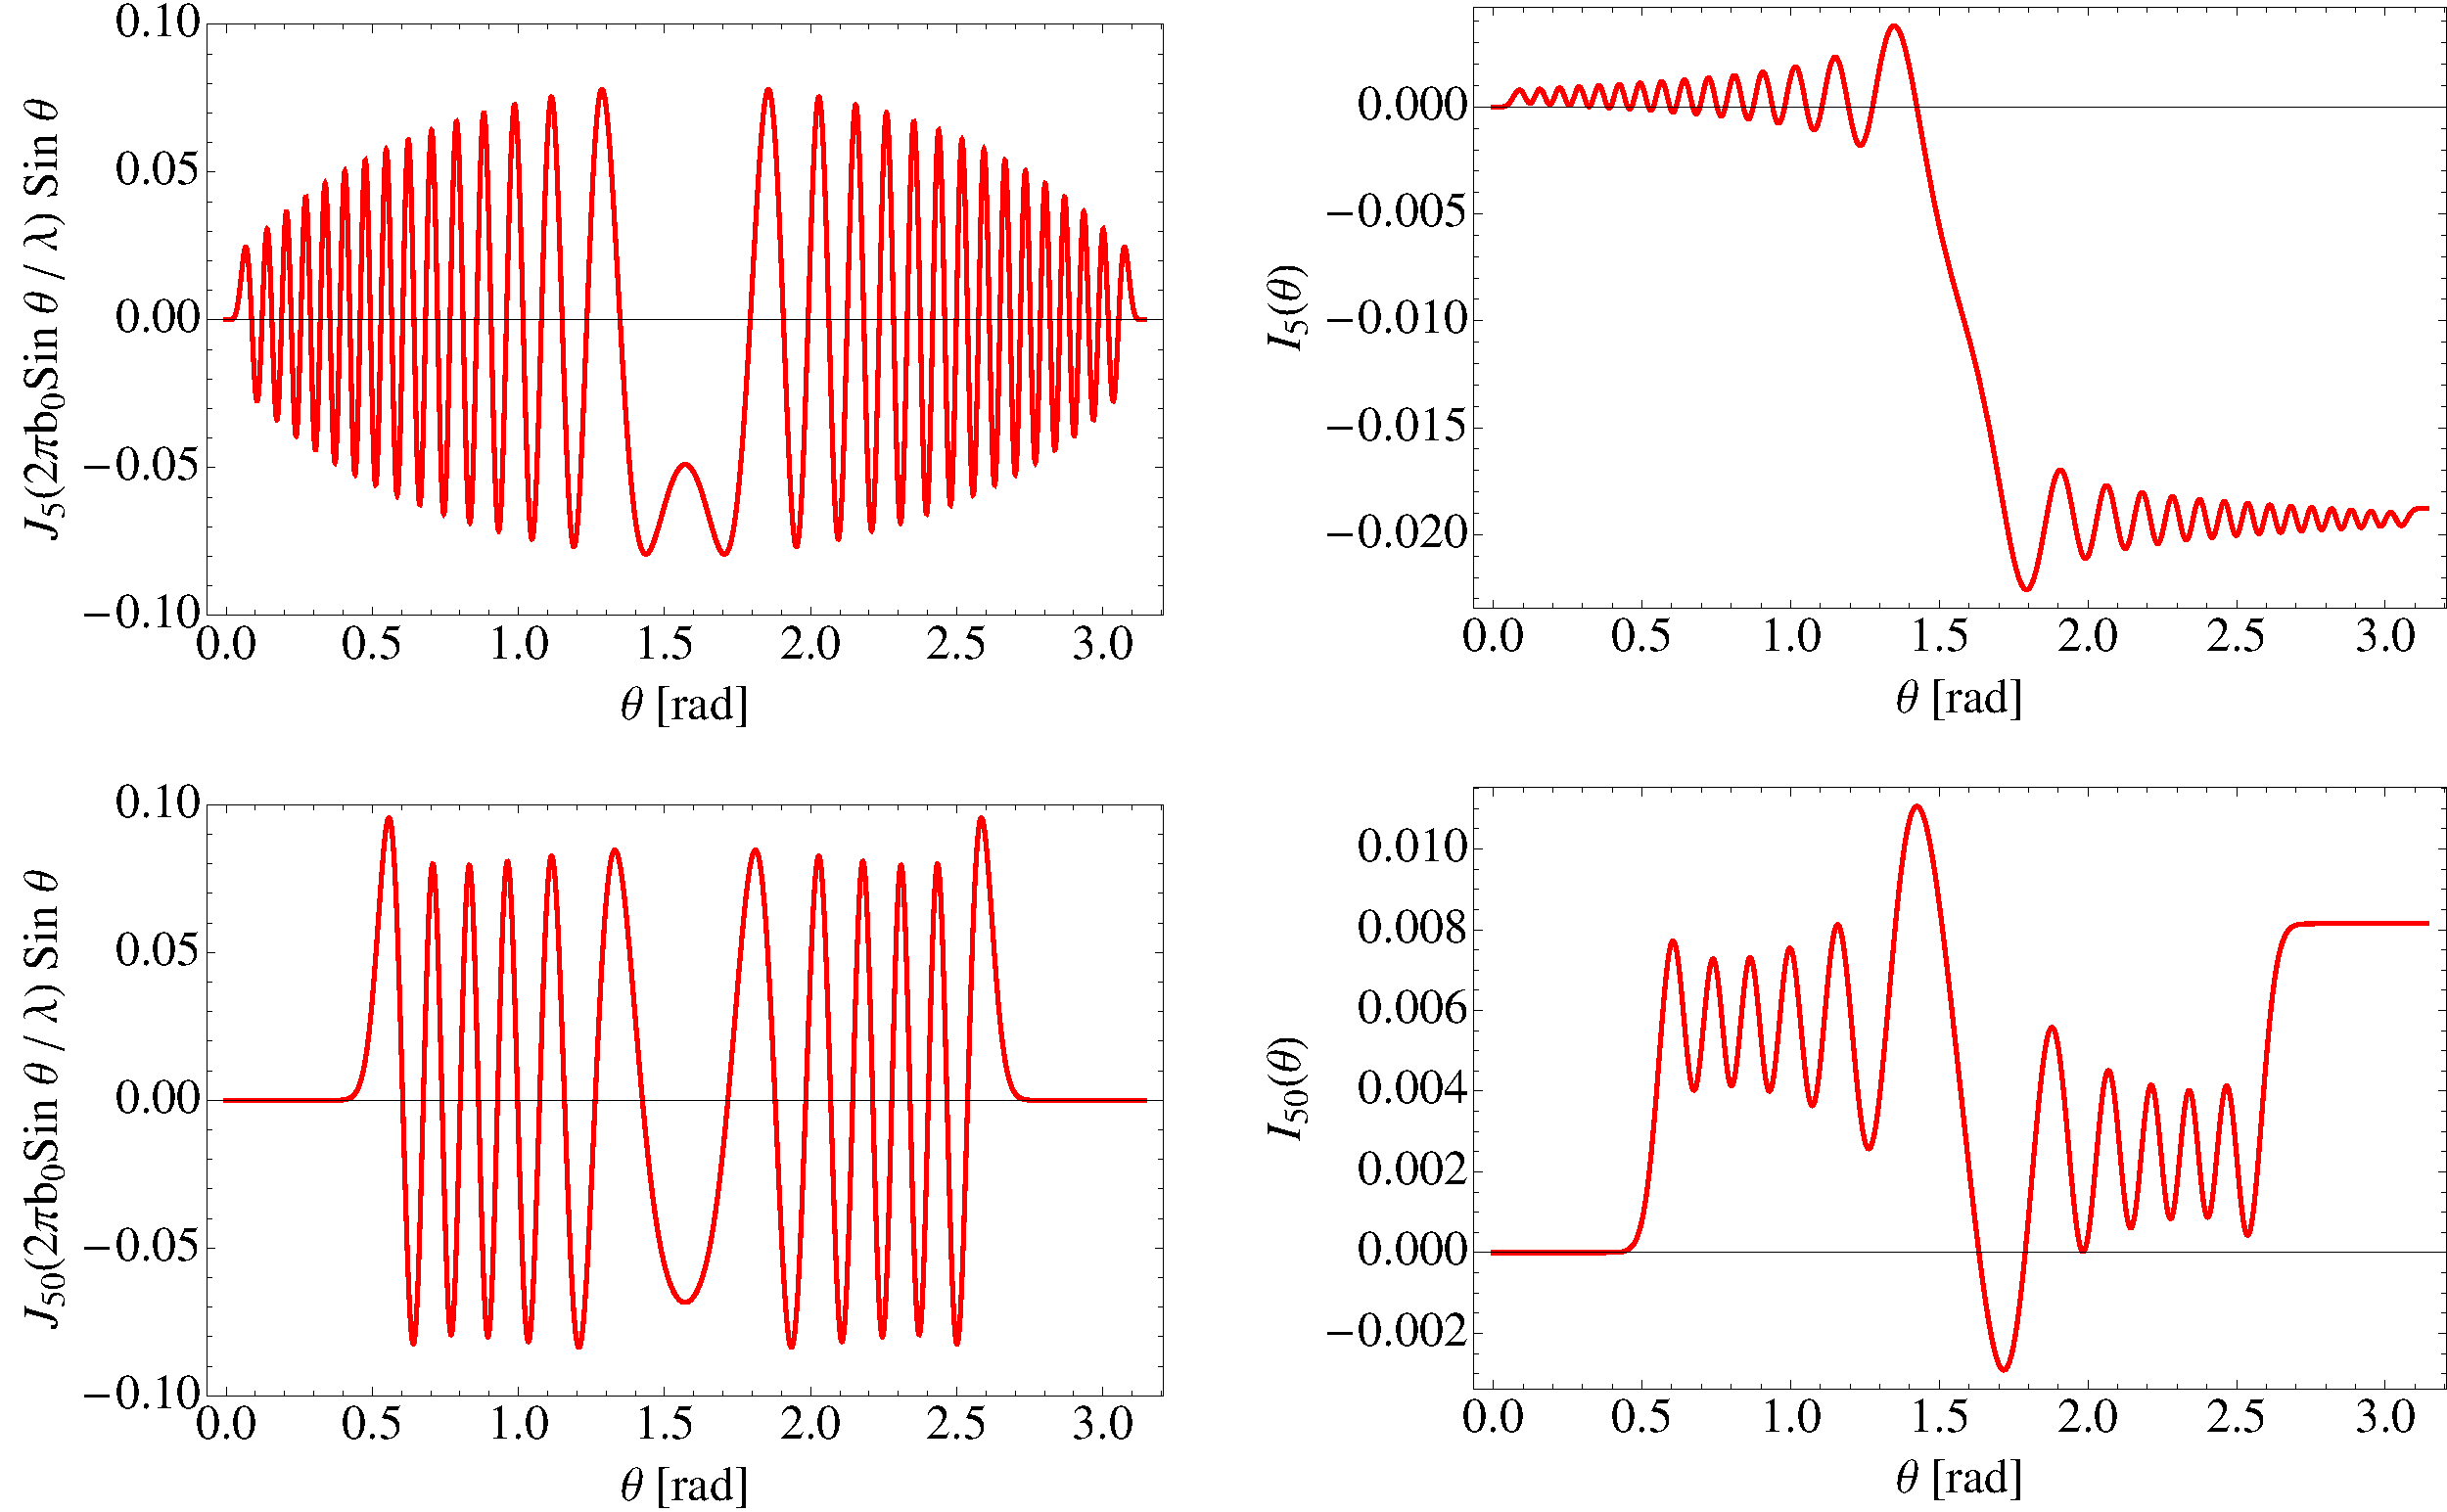
\includegraphics[width=1.0\textwidth]{plots/besselContributions.pdf}
%\caption{
%Left column: responses of selected fringe rate bins to different $\theta$ (and
%therefore different declinations).  Right column: cumulative response
%integrated from $0$ to $\theta$, i.e. $I_n (\theta)$ as defined by Equation
%\eqref{eq:cumulResponse}.  The top row shows the $n=5$ fringe-rate bin, while
%the bottom row shows the $n=50$ fringe-rate bin, with the $n^{th}$ bin defined
%to have a fringe rate of $f_n \equiv n / T_\Earth$.  For these illustrative
%plots, the primary beam was ignored, and the baseline under consideration was a
%single $16\lambda$ baseline with an east-west orientation at the equator.  From
%the right column, one sees that lower fringe rates derive most of their
%celestial signal from a narrow region in the sky, so low-pass fringe-rate
%filtering suggested in Section \ref{fringeRateIntro} causes a narrowing of the
%effective primary beam.
%}
%\label{besselContributions}
%\end{figure*}

\section{Combining time-ordered data without mapmaking}
Until now, our discussion of fringe-rate filtering has centered around the mapmaking problem.  However, our intuitive understanding of fringe-rate filtering---that it differentiates instrumental noise from celestial signals by identifying high fringe-rates as being noise-dominated---holds much more generally.    In this section, we show how fringe-rate filtering can be used a de-noising tool for visibilities, bypassing the image domain entirely.  This allows one to take advantage an important benefit of mapmaking, namely, the reduction of instrumental noise through the coherent combination of time-ordered data, while avoiding some of its drawbacks such as the introduction of curved-sky or gridding artifacts.  Moreover, for many applications (such as power spectrum estimation), it is more natural to work with interferometric visibilities directly, provided they can be de-noised.

To de-noise our visibilities, suppose (for a brief moment) that one did in fact produce an estimator $\xhat$ of the sky in the image domain.  One could then transform this estimator back into time-ordered visibilities $\vis_\textrm{filt}$ by simply computing $\vis_\textrm{filt} \equiv \A \xhat$.  Such a set of visibilities would represent de-noised visibilities since Equation \eqref{optEst} is essentially a best-fit solution based on noisy data, which means that $\A \xhat$ is simply the predicted measurements from the best-fit model.  Now, if these predicted measurements were actually generated by first forming a map, one would still incur all the difficulties in imaging that one had hoped to avoid.  To deal with this issue, we note that the relationship between the original visibilities and the de-noised ones are given by
\begin{equation}
\vis_\textrm{filt} = \A \left[ \A^\dagger \N^{-1} \A \right]^{-1} \A^\dagger \N^{-1} \vis \equiv \mathbf{W}  \vis.
\end{equation}
The matrix $\mathbf{W}$ can be thought of as a de-noising filter, and if it can be computed analytically we will have bypassed imaging entirely.

Fortunately, an analytic treatment is possible if one makes the observation that the matrices ``internal" to $\mathbf{W}$ can be expressed in any basis without affecting the final result.  Expressing the $\A$ matrix in a fringe-rate/azimuthal Fourier mode/polar angle/baseline basis, i.e. the basis implied by Equation \eqref{eq:convenientBasis}, a little algebra reveals that $\mathbf{W}$ takes the form
\begin{equation}
\label{eq:denoiseweights}
\mathbf{W}_{n,b; n^\prime\!,b^\prime} = \delta_{nn^\prime}\sum_{b^{\prime\prime}} \frac{c_{bb^\prime}(n) c^*_{b^\prime b^{\prime\prime}}(n)}{(\lambda_{b^{\prime \prime}}^n )^2},
\end{equation}
where we have again assumed white noise, and have defined
\begin{equation}
c_{bb^\prime}(n) \equiv  \int_0^\pi  g_b^*(\theta,n) g_{b^{\prime}}(\theta,n) d\theta.
\end{equation}
[XXX: may need to be clearer about what basis the final result is in.]  The various matrix elements of $\mathbf{W}$ provide the linear combinations of data from various baselines and fringe-rate bins that should be taken to de-noise the data.  Different fringe-rate bins do not mix, whereas the data from different baselines are combined to de-noise a given fringe-rate bin.  Intuitively, a given fringe-rate is measured by different baselines with different levels of sensitivity (for instance, longer baselines more ``naturally" sample higher fringe-rates), and $\mathbf{W}$ takes this into account to combine data in an optimal way.  Note that with our analytical prescription, all relevant quantities can be precomputed given a beam model, and no imaging is required to combine information from different baselines.

\subsection{De-noising visibilities from a single baseline}

While Equation \eqref{eq:denoiseweights} is useful for combining information from different baselines, it is unable to de-noise data from a single baseline.  Indeed, one can see that $\mathbf{W}$ reduces to the identity matrix in the single baseline case.  To understand this, recall that for a drift-scan interferometer there is a one-to-one, monotonic correspondence fringe-rate and azimuthal Fourier number.  Thus, while high fringe-rate bins are quite \emph{likely} to be noise-dominated, if the sky contained a strong signal in a high azimuthal Fourier mode, it would in principle be \emph{possible} for the bin to be signal-dominated.  Put another way, high fringe-rate bins are not necessarily noise-dominated and discardable, since they each access unique information about the sky.

In order to de-noise visibilities from a single baseline, it is necessary to place a prior on the nature of the sky signal.  For instance, suppose one had reliable prior knowledge of the sky in the form of a signal covariance matrix $\mathbf{S} \equiv \langle \x \x \rangle$.  One could then form a Wiener-filtered estimate of $\x$:
\begin{equation}
\label{eq:WienerEst}
\xhat_\textrm{Wiener} = \left[ \mathbf{S}^{-1} + \mathbf{A}^\dagger \mathbf{N}^{-1} \mathbf{A} \right]^{-1} \mathbf{A}^\dagger \mathbf{N}^{-1} \vis,
\end{equation}
which by construction minimizes $\langle | \xhat_\textrm{Wiener} - \x |^2 \rangle$, the expected error \citep{Tegmark97}.  Like before, we can then proceed to multiply by $\mathbf{A}$ to arrive at a set of filtered visibilities:
\begin{equation}
\vis_\textrm{Wiener} \equiv \A \xhat_\textrm{Wiener}.
\end{equation}
As an example, suppose the sky consisted of a continuum of unresolved and unclustered point sources.  The signal covariance matrix would then be of the form $\mathbf{S} = \sigma_s^2 \mathbf{I}$, where $\sigma_s$ is some root-mean-square signal magnitude.  In the low signal-to-noise limit\footnote{What turns out to be a signal-to-noise weighting in our special case simply becomes a signal-over-signal-plus-noise weighting in the general case.}, where the second term in Equation \ref{eq:WienerEst}'s inverse term can be neglected, the de-noising filter $\mathbf{W}^\textrm{Wiener}$ becomes
\begin{equation}
\label{eq:WienerWeights}
\mathbf{W}^\textrm{Wiener}_{n n^\prime} = \delta_{n n^\prime} \frac{\sigma_s^2}{\sigma_n^2} \int_0^{\pi}  | g_b (\theta, n) |^2 d\theta.
\end{equation}
Each element of this diagonal matrix specifies a weighting for a fringe-rate bin.  The integral quantifies the response of the baseline to the particular fringe-rate bin, and when multiplied by $\sigma_s^2$, gives the signal in the bin.  (Note that $\sigma_s$ and $\sigma_n$ have different units, so that $\mathbf{W}^\textrm{Wiener}$ is dimensionless).  With $\sigma_n^2$ in the denominator, the Wiener filter enacts a signal-to-noise weighting in fringe-rate space.  Given that $ | g_b (\theta, n) |^2$ decays rapidly at high $n$ (as discussed in previous sections), the Wiener filter does precisely what we intuitively expect it to do: it down-weights high fringe-rates that are likely noise-dominated.  Our placement of a flat signal prior essentially precluded the possibility that a strong signal in high azimuthal Fourier modes could result in a signal-dominated measurement at high fringe-rate bins, allowing us to safely downweight those bins without sacrificing signal.

Care must be taken, however, when using a set of visibilities that have been Wiener-filtered.  Because fringe-rate filtering is effectively a way to enact time-integration, the resulting time-series of filtered visibilities will possess correlated errors and will no longer be independent.  This is expected and desirable in the sense that it is what allows the Wiener filter to minimize errors.  However, this comes at a cost.  Recall that fringe-rates map directly to azimuthal Fourier mode numbers.  Thus, if one were to use the Wiener-filtered data to measure (say) a power spectrum, the result would be biased low, as Equation \eqref{eq:WienerWeights} gives fringe-rate weights that are all less than one.  Instead, we envision the Wiener-filtered visibilities as one where the lower noise levels allow systematics to be more clearly identified.\footnote{It is admittedly possible to construct an unbiased power spectrum estimator from Wiener-filtered visibilities: one simply renormalizes any fringe-rate bins that were biased low by the Wiener-filter.  The only subtlety is that this renormalization cannot be performed individually on different fringe-rate bins, since the diagonal nature of $\mathbf{W}^\textrm{Wiener}$ would result in the identity matrix.  Instead, we must make the observation that a typical power spectrum estimator takes advantage of statistical isotropy to sum together the power estimates of individual azimuthal modes (or equivalently, fringe rates) to form power estimates on a particular angular scale.  As long as the final estimate on each angular scale is properly normalized, the result will be unbiased.  However, it will not be \emph{optimal} (unlike the estimator that we will derive in Section \ref{sec:OptPower}) in the sense that the error bars will not be as small as can be possibly achieved by the data set.}

\section{Power Spectrum Estimation with Fringe-Rate Filtering}
\label{sec:OptPower}
We now discuss the problem of power spectrum estimation given time-ordered data.  The primary challenge, again, is to ensure that the benefits of a long time-integration (i.e. increased sensitivity) can be realized without explicitly making maps.  For example, one cannot simply average over power spectrum estimates formed from every time instant of some time-ordered visibilities.  Doing so would reduce the sensitivity of the final power spectrum, as coherent information between time-samples would be lost.  However, it would be desirable to be able to optimally include coherent information while remaining in a time-ordered basis where systematic effects are transparent.  In this section, we will show that the techniques of fringe-rate filtering make it possible to construct a power spectrum estimator that satisfies these requirements.

We start with the estimator $\hat{p}_\alpha$ for the $\alpha$th band of the power spectrum:
\begin{equation}
\label{eq:GenFormPowEst}
\hat{p}_\alpha = N_\alpha \hat{\x}^\dagger \mathbf{C}^{-1} \mathbf{Q}_\alpha \mathbf{C}^{-1} \hat{\x},
\end{equation}
where $\mathbf{C} \equiv \langle \hat{\x} \hat{\x}^\dagger \rangle = \mathbf{S} + \boldsymbol \Sigma$ is the \emph{total} (signal plus noise) covariance matrix of the sky map, and $N_\alpha$ is a normalization factor, given by\footnote{More sophisticated normalization schemes involving matrix normalization constants are possible [XXX: cite Josh MWA paper], but for simplicity (and no loss of generality as far as our present discussion is concerned) we do not consider them here.}
\begin{equation}
N_\alpha = \textrm{tr} \left[ \mathbf{C}^{-1} \mathbf{Q}_\alpha \mathbf{C}^{-1} \mathbf{Q}_\alpha \right].
\end{equation}
[XXX: grr...the Fisher matrix isn't diagonal here, so it's a little more annoying when it comes to normalization.  Need to decide which norm convention to use].  Written in this general form, our estimator can be used to estimate any power spectrum, be it an angular power spectrum $C_\ell$ (in which case $\hat{p}_\alpha \equiv \hat{C}_\ell$ and $\alpha$ would index the $\ell$ value), or a three-dimensional power spectrum $P(\mathbf{k} )$ (in which case $\hat{p}_\alpha \equiv \hat{P}(\mathbf{k}_\alpha)$).  The type of power spectrum under consideration is encoded by the form of the $\mathbf{Q}_\alpha$ matrices.  They are defined as the linear response of the covariance matrix $\mathbf{C}$ to the power spectrum:
\begin{equation}
\mathbf{Q}_\alpha \equiv \frac{\partial \mathbf{C}}{\partial p_\alpha}.
\end{equation}
The inverse-covariance weighting enacted by $\mathbf{C}^{-1}$ makes Equation \eqref{eq:GenFormPowEst} a minimum-variance estimator \citep{liu_tegmark2011}.  For notational cleanliness we have omitted any corrections to \emph{additive} biases in the estimator, implicitly assuming that such biases have already been removed.

As it stands, our estimator is written explicitly in terms of the estimated sky maps $\hat{\x}$.  These are related to the visibilities via Equation \eqref{optEst}, which states that $\xhat = \left[ \A^\dagger \N^{-1} \A \right]^{-1} \A^\dagger \N^{-1} \vis$.  If we assume that our measurements are noise-dominated, then $\mathbf{C} \approx \boldsymbol \Sigma = [ \mathbf{A}^\dagger \mathbf{N}^{-1} \mathbf{A} ]^{-1}$, so $\mathbf{C}^{-1} \approx [ \mathbf{A}^\dagger \mathbf{N}^{-1} \mathbf{A} ]$.  Inserting these into Equation \eqref{eq:GenFormPowEst}, we obtain
\begin{equation}
\label{eq:VisBasedPowEst}
\hat{p}_\alpha = N_\alpha \hat{\vis}^\dagger \N^{-1} \A  \mathbf{Q}_\alpha \A^\dagger \N^{-1} \vis
\end{equation}
as our visibility-based estimator.

To see how fringe-rate filters relate to this expression, consider the specific example of measuring the angular power spectrum $C_\ell$.  In this case, we parameterize the signal covariance in terms of spherical harmonics, so that
\begin{equation}
\mathbf{C}_{\hat{\r}, \hat{\r}^\prime} = [ \mathbf{A}^\dagger \mathbf{N}^{-1} \mathbf{A} ]^{-1} + \sum_{\ell m} Y_{\ell m} ( \hat{\r}) Y^*_{\ell m} (\hat{\r}^\prime) C_\ell,
\end{equation}
and thus
\begin{equation}
\label{eq:CEllQ}
\mathbf{Q}_\ell \equiv \frac{\partial \mathbf{C}}{\partial C_\ell} = \sum_{m} Y_{\ell m} ( \hat{\r}) Y^*_{\ell m} (\hat{\r}^\prime),
\end{equation}
where we have renamed the index $\alpha$ to $\ell$ as a reminder that we are considering the angular power spectrum.  Note that since the noise covariance does not depend on the power spectrum $C_\ell$, it is necessary to include the signal covariance when deriving $\mathbf{Q}_\ell$, even though this was unnecessary for $\mathbf{C}^{-1}$.

Substituting Equations \eqref{eq:AdagNinvv} and \eqref{eq:CEllQ} into Equation \eqref{eq:VisBasedPowEst}, we obtain
\begin{equation}
\label{eq:StillFringe}
\widehat{C}_\ell \propto \sum _{m=-\infty}^\infty \Bigg{|} \sum_b w_{\ell m}^b \widetilde{V}_b (f_m) \Bigg{|}^2,
\end{equation}
where
\begin{equation}
w_{\ell m}^b \equiv
\begin{cases}
2 \pi \int d(\cos \theta) N_{\ell}^m P_{\ell}^{m} (\cos \theta) g_b(\theta,m),& \textrm{for} -\ell \leq m \leq \ell \\
0, & \textrm{otherwise,}
\end{cases}
\end{equation}
with $P_\ell^m$ being the associated Legendre polynomial of order [XXX: insert proper name here], and
\begin{equation}
N_\ell^m = \sqrt{\frac{2\ell + 1}{4 \pi} \frac{(\ell-m)!}{(\ell + m )!}}
\end{equation}
is the normalization constant for spherical harmonics.  Since we can equivalently interpret $m$ not as the azimuthal Fourier mode number but as the fringe-rate bin index, it is the Fourier dual to time, our estimator can be rewritten using Parseval's theorem:
\begin{equation}
\label{eq:FinalTimeEst}
\widehat{C}_\ell \propto  \int_{-T_\Earth / 2}^{T_\Earth /2} \frac{dt}{T_\Earth} \Bigg{|} \sum_b V^\textrm{filt}_{\ell b} (t) \Bigg{|}^2,
\end{equation}
where
\begin{equation}
\label{eq:FinalFilt}
V^\textrm{filt}_{\ell b} (t) \equiv  \sum_m \exp \left[i \frac{2 \pi m t}{T_\Earth}\right]  w_{\ell m}^b \widetilde{V}_b (f_m).
\end{equation}
Together, Equations \ref{eq:FinalTimeEst} and \ref{eq:FinalFilt} suggest a method for estimating power spectra.  First, time-ordered visibilities are Fourier-transformed into a fringe-rate basis.  Different fringe-rate bins are then weighted by the $w_{\ell m}^b$ weights, which essentially encode the ``dot product" between a baseline's response in the fringe-rate bin and the angular mode in question.  The result is then transformed back into a set of fringe-rate filtered visibility time series.  A power spectrum is computed for every time instant before averaging together different times.  Since this procedure was derived from a minimum-variance estimator of the power spectrum, it is guaranteed to produce the smallest possible error bars.

We have thus accomplished our goal of writing down an optimal estimator for the power spectrum that works directly with visibilities.  Conveniently, the integration of coherent information takes place via a fringe-rate filter, which operates on independently for different baselines.  Moreover, since it returns data in its original format---a time-series---systematics localized to certain baselines and certain times can be easily isolated.  Note that while the filtering is performed per-baseline, information from multiple baselines regarding the same $\ell$ mode is coherently included before squaring to form the power spectrum.  This is most clearly seen in Equation \eqref{eq:StillFringe}, where visibilities from different baselines are simply added together, except that they are weighted by different amounts depending on how much overlap they have with the mode in question.  Traditionally, taking advantage of coherent information between non-identical baselines requires imaging (whether in the image basis or as a Fourier-transformed image in the form of, say, $uv$-plane data).  With our approach, imaging (and its attendant artifacts) are completely avoided without sacrificing sensitivity.
[XXX: JUST REALIZED THIS IS FAR MORE ALGORITHMICALLY EFFICIENT THAN MAPMAKING!!!]

[XXX: Maybe also consider $l \sim 2 \pi b / \lambda$ approx.]
[XXX: Perhaps make connection to thingy more clear.]
[XXX: Consider also playing up the weights as the ``dot product" of the thing you're interested in and the fringe-rate-space visibilities to emphasize how different baselines just need to combined based on their overlap.]
%
%One approach to forming an estimate of the power spectrum would be to start from the Wiener-filtered visibilities from the previous section.  As mentioned above, however, doing so would result in a power spectrum that contained a multiplicative bias.  A straightforward fix to this problem would be to appropriately normalize the Wiener weights derived in Equation \eqref{eq:WienerWeights}.  Roughly speaking, those fringe-rates that were biased low by the Wiener filter can simply be renormalized to the appropriate level.  We caution, however, that this renormalization cannot be done on a fringe-rate-by-fringe-rate basis, since the diagonal nature of $\mathbf{W}^\textrm{Wiener}$ would result in the identity matrix.  (This follows immediately from the arguments that led us to impose a prior on the signal covariance matrix, namely that each fringe-rate bin probes unique information on the sky).  However, a typical power spectrum estimator takes advantage of statistical isotropy to sum together the power estimates of individual azimuthal modes (or equivalently, fringe rates).  To arrive at a power-conserving normalization, then, we simply require that the summed power estimates are properly normalized.  This allows different fringe rates to retain their relative normalization, preserving the de-noising ability of our filter.   [	XXX: should we explicitly construct the sub-optimal Wiener-filter-based estimator?]
%
%While the aforementioned procedure will indeed result in an unbiased power spectrum estimator, 
%
%Before deriving the correct normalization factors, we first pause to discuss the optimality of this procedure.   At first glance, the normalized Wiener-filter that we just described is not guaranteed to be an optimal way to estimate the power spectrum (in the sense of producing minimum-variance power spectrum estimates), since the Wiener filter was constructed only to minimize errors in images.  We will now show, however, that in the low signal-to-noise regime discussed above, the procedure is in fact optimal, and is derivable from an optimal power spectrum estimator.  We start with the estimator $\hat{p}_\alpha$ for $P(k_\alpha)$:
%\begin{equation}
%\hat{p}_\alpha = N_\alpha \hat{\x}^\dagger \mathbf{C}^{-1} \mathbf{Q}_\alpha \mathbf{C}^{-1} \hat{\x},
%\end{equation}
%where $\mathbf{C} \equiv \langle \hat{\x} \hat{\x}^\dagger \rangle = \mathbf{S} + \boldsymbol \Sigma$ is the \emph{total} (signal plus noise) covariance matrix of the sky map, and $N_\alpha$ is a normalization factor.  The inverse-covariance weighting enacted by $\mathbf{C}^{-1}$ makes this a minimum-variance estimator \citep{liu_tegmark2011}, and for notational cleanliness we have omitted any corrections to \emph{additive} biases in the estimator, implicitly assuming that such biases have already been removed.  \cite{seljak1998} showed that this estimator can easily rewritten in terms of the Wiener-filtered estimator for the sky:
%\begin{eqnarray}
%\label{eq:WienerPowerEst}
%\hat{p}_\alpha &=& N_\alpha \hat{\x}^\dagger_\textrm{Wiener} \mathbf{S}^{-1} \mathbf{Q}_\alpha \mathbf{S}^{-1} \hat{\x}_\textrm{Wiener} \nonumber \\
%&=& N_\alpha \hat{\x}^\dagger_\textrm{Wiener}  \mathbf{Q}_\alpha \hat{\x}_\textrm{Wiener},
%\end{eqnarray}
%where in the second equality we assumed, like before, that $\mathbf{S} = \sigma_s^2 \mathbf{I}$ and absorbed the $\sigma_s^2$ into the normalization.  As it currently stands, the power spectrum estimator takes maps (whether Wiener filtered or not) as input.  In a similar spirit to the previous section, we would prefer to evade imaging artifacts by working directly from visibilities.  To rewrite Equation \eqref{eq:WienerPowerEst}, we make use of the following trick.  Working from Equation \eqref{manifest}, it is clear that
%\begin{equation}
%(\mathbf{A}^\dagger \mathbf{A} )_{m, \theta ; m^\prime \theta^\prime} = \delta_{mm^\prime} g_b(\theta, m) g_b^*(\theta^\prime, m^\prime).
%\end{equation}
%Suppose we apply this operator to $\hat{\x}_\textrm{Wiener}$ (the motivation for this will become clear momentarily), which we can express as 
%\begin{equation}
%\xhat_\textrm{Wiener} = \frac{\sigma_s^2}{\sigma_n^2} \mathbf{A}^\dagger  \vis,
%\end{equation}
%
%
%This process---first Wiener-filtering and then 
%
%[XXX: Discuss the assumptions made.]
%
%As an example, suppose one were to form an estimator of the angular cross-power spectrum $C_\ell$ between the sky at two frequencies:
%\begin{equation}
%\label{eq:C_Ell}
%\widehat{C}_\ell (\nu, \nu^\prime) \propto \frac{1}{2\ell + 1} \sum_{m=-\ell}^{\ell} \vis^*_m (\nu) \vis_m (\nu^\prime),
%\end{equation}
%where $K=...$ [XXX: put in a conversion factor for Jy to K etc. Need to be better about the distinction between xhat and v].  If one makes the assumption that a given baseline's response is strongly peaked at the specific angular mode $\ell \sim 2 \pi \sqrt{b_x^2+ b_y^2} / \lambda$, we will only need to consider the estimator on a baseline-by-baseline basis.  If the input visibilities are chosen to be the Wiener-filtered ones, this estimator can be shown to be an optimal, minimum-variance estimator [XXX: need to dig up Ue-Li and Uros' paper references].  Now, isotropy dictates that all azimuthal Fourier modes contribute the same power.  To ensure that the power spectrum estimate is properly normalized, we therefore require the \emph{square} of the weights given by Equation \eqref{eq:WienerWeights} sum to unity.  In other words, for the purposes of power spectrum estimation one weights the $n^\textrm{th}$ fringe-rate bin by
%\begin{equation}
%w_n = \frac{ \int_0^{\pi}  | g_b (\theta, n) |^2 d\theta}{\sum_m \left( \int_0^{\pi}  | g_b (\theta^\prime, m) |^2 d\theta^\prime \right)^2 },
%\end{equation}
%with filtered visibilities given by $v^\textrm{filt}_n = w_n v_n$.
%
%Equation \eqref{eq:C_Ell} can be written in terms of a time-series by the nothing the following.  Since the interferometer response decays rapidly for large fringe-rate bins, we can extend the sum over $m$ to go from $-\infty$ to $+\infty$.  Then recalling that $m$ doubles as the fringe-rate index, which is the Fourier dual to time, one can use Parseval's theorem to write
%\begin{equation}
%\widehat{C}_\ell \propto \frac{1}{2\ell +1}  \int_{-\frac{T_\Earth}{2}}^{\frac{T_\Earth}{2}} \frac{dt}{T_\Earth}   V_{\textrm{filt}}^* (\nu,t) V_\textrm{filt} (\nu^\prime,t),
%\end{equation}
%where
%\begin{equation}
%V_\textrm{filt}(\nu,t)=  \sum_m \exp \left[i \frac{2 \pi m t}{T_\Earth}\right] w_m v_m (\nu).
%\end{equation}
%Written in this way, it is clear that the optimal power spectrum estimator reduces to averaging together estimators that are formed at every instant in time---provided that one uses the fringe-rate filtered visibilities instead of the original, unprocessed visibilities.  Ordinarily, forming power spectra at every instant is suboptimal because it involves the squaring of visibilities, resulting in the loss of coherent phase information.  In other words, one cannot coherently add together constraints on the same sky information from different time slices, and errors in the power spectrum average down as $1/\sqrt{t}$.  Traditionally, coherent integration is implemented by first forming a map of the sky (in whatever basis one desires), and then to estimate the power spectrum from the maps.  The final errors on the power spectrum then decrease as $1/t$.  What has been shown here is that fringe-rate filtered visibilities are visibilities that have effectively already been coherently integrated in time, and estimating the power spectrum time-slice-by-time-slice with them represents no loss of sensitivity.  Working in a time basis can be preferable to using Equation \eqref{eq:C_Ell} directly because many systematics can be more easily isolated by examining time-series data.  Our analytic expressions allow fringe-rate filtering to be performed without mapmaking, reducing the possibility of image-domain artifacts and curved-sky complications.
%
[XXX: Need to find a place to talk about effective beams and how it affects power spectrum sensitivity.  Talk about how we will henceforth use simulated effective beams so that we don't have to make all the assumptions that went into the analytic work.  Should also credit Richard for the fringe-rate --> m-mode correspondence more throughout.]


%While we established in the previous section that Wiener-filtered visibilities would give biased estimates of the power spectrum, we can fortunately sidestep the problem by making a different assumption---that of isotropy.
%
%To pick a concrete example that will serve as the focus for the rest of the paper, consider the power spectrum $P(\mathbf{k})$ of highly redshifted $21\,\textrm{cm}$ emission.  At each instant, spatial fluctuations that are perpendicular to the line-of-sight are probed by the fringe-patterns of a baseline, while the spectral nature of the measurement means that structure along the line-of-sight is accessed by the frequency spectrum of the visibilities.  Specifically, if one performs a delay transform on a baseline's visibility by Fourier transforming its frequency spectrum (thus expressing the spectrum in delay space), the result is a probe of the Fourier mode with wavevector $\mathbf{k} \approx 2 \pi (b_x / \lambda X, b_y / \lambda X, \tau /Y)$, where $b_x$ and $b_y$ are the x- and y-components of the baseline vector, respectively, $\tau$ is the delay.  The scalars $X$ and $Y$ convert angles and frequency to comoving distances, respectively.  In the limit that the baseline in question is short (which is typical of many $21\,\textrm{cm}$ experiments such as PAPER), the approximation that the delay-transformed visibility probes a single Fourier mode on the sky becomes an excellent one, with the response of a baseline becoming sharply peaked at the $\mathbf{k}$ value quoted above \citep{P12b}.  Given this, an estimator $\widehat{P} (\mathbf{k})$ for the power spectrum can be computed from a single baseline and a single time instant:
%\begin{equation}
%\widehat{P} (\mathbf{k}) = \left( \frac{\lambda^2}{2 k_B} \right)^2 \frac{X^2 Y}{\Omega B} \big{|} \overline{V}_{\mathbf{b}}(\tau) \big{|}^2,
%\end{equation}
%where $B$ is the bandwidth, $k_B$ is Boltzmann's constant, $\overline{V}_{\mathbf{b}}$ is the delay-transformed visibility from baseline $\mathbf{b}$, and it is understood that the $\mathbf{k}$ mode being probed is the one corresponding to the values of $\mathbf{b}$ and $\tau$.
%
%To reduce errors on a measured power spectrum, one can take advantage of isotropy, summing together power spectrum estimates with the same wavenumber $k \equiv |\mathbf{k}|$.  With our assumption of short baselines, the wavenumber is dominated by the contribution from $\tau$, and changing the azimuthal Fourier number $m$ represents a negligible difference in the $k$ mode being probed.  We may therefore reduce errors in our power spectrum estimate by summing over estimates formed from treating different $m$ modes individually.  For a minimum-variance treatment, the input visibilities must be inverse covariance weighted prior to squaring, and more formally, one can write the estimator of an unnormalized power spectrum $q(k)$ as \citep{liu_tegmark2011}
%\begin{equation}
%q(k) = \vis^\dagger \mathbf{C}^{-1} \mathbf{Q}(k) \mathbf{C}^{-1} \vis,
%\end{equation}
%where $\mathbf{C}$ is the \emph{total} (signal + noise) covariance of the visibilities, given by
%\begin{equation}
%\mathbf{C} = \A \mathbf{S} \A^\dagger + \N,
%\end{equation}
%and $\mathbf{Q} (k)$ is the response of the covariance to the power spectrum at wavenumber $k$, i.e.
%\begin{equation}
%\mathbf{Q} (k) \equiv \frac{\partial \mathbf{C}}{\partial P(k)} = \A \frac{\partial \mathbf{S}}{\partial P(k)} \A^\dagger,
%\end{equation}
%where in the last equality we made use of the fact that neither the noise $\N$ nor the instrumental response $\A$ depend on the cosmological power spectrum.
%
%Explicitly, in spatial Fourier space the signal covariance $\mathbf{S}$ is diagonal with diagonal elements proportional to the power spectrum:
%\begin{eqnarray}
%\mathbf{S}_{\mathbf{k},\mathbf{k}^\prime} &=& \frac{\Omega B}{X^2Y} \left( \frac{2k_B}{\lambda^2}\right)^2 P(k) \delta_{\mathbf{k},\mathbf{k}^\prime} \nonumber \\
%& \approx &  \frac{\Omega B}{X^2Y} \left( \frac{2k_B}{\lambda^2}\right)^2 P(k) \delta_{k,2\pi\tau/Y}  \delta_{k,k^\prime} \delta_{b b^\prime} \delta_{m m^\prime}, \qquad
%\end{eqnarray}
%where in the last equality we have made several assumptions.  First was the assumption stated previously, that $k$ is dominated by the contribution along the line-of-sight (i.e. from $\tau$).  For the wavenumber component perpendicular to the line of sight, $k_\perp$ 
%Effective beams
%
%\subsection{De-noising data sets for power spectrum estimation}
%Until now, our discussion of fringe-rate filtering has centered around the mapmaking problem.  However, our intuitive understanding of fringe-rate filtering---that it differentiates instrumental noise from celestial signals by identifying certain fringe rates as being too rapid to be physical sources on the sky---holds much more generally.  In this section, we consider fringe-rate filtering in the context of power spectrum estimation, and in particular show how fringe-rate filtering can be used as a preprocessing tool to de-noise data sets prior to power spectrum estimation.
%
%Our goal is to consider how an optimal estimator for a power spectrum (or any other two-point statistic) can be phrased in terms of a fringe-rate filtered data set.  As an example, we will consider the frequency-frequency angular cross-power spectrum $C_\ell (\nu, \nu^\prime)$.  This represents no loss of generality, even though most $21\,\textrm{cm}$ experiments seek to measure the spherically averaged power spectrum $P(k)$, as the two quantities are related by an invertible linear operation (which we show explicitly in Appendix XXX).  Thus, an optimal and lossless prescription for computing $C_\ell (\nu, \nu^\prime)$ can be easily translated into one for $P(k)$.  Here we deal with the former because it is a more natural quantity to consider when the flat-sky approximation does not hold.
%
%To form an optimal estimator for $C_\ell (\nu, \nu^\prime)$, one computes
%\begin{equation}
%\label{eq:generalEst}
%\widehat{C}_\ell (\nu, \nu^\prime)  = N_\ell \vis^\dagger(\nu) \mathbf{C}^{-1} \mathbf{Q}^\ell \mathbf{C}^{-1} \vis(\nu^\prime),
%\end{equation}
%where $\mathbf{C} \equiv \langle \vis \vis^\dagger \rangle$ is the covariance matrix of measured visibilities, $\mathbf{Q}^\ell \equiv \partial \mathbf{C} / \partial C_\ell $ is the response of the covariance matrix to $C_\ell$, and $N_\ell$ is a normalization constant.  [XXX: cite stuff].  As usual, this matrix equation can be evaluated in any basis.  Like before, however, it will be particularly convenient to express the relevant measurements in a per-baseline, fringe-rate basis, and the true sky in terms of spherical harmonics so that $T(\rhat) = \sum_{\ell m} a_{\ell m} Y_{\ell m} (\rhat)$.  Re-expressing our measurement equation yet again, we have
%\begin{equation}
%\widetilde{V}_b (f_m) = \sum_\ell w_{\ell m} (b) a_{\ell m} + n_{m}
%\end{equation}
%where
%\begin{eqnarray}
%w_{\ell m} = \sum_n \int d\Omega && Y_{\ell n}^*(\rhat) e^{i \frac{2 \pi b_y}{\lambda} \cos \eta \cos \theta} e^{i m \varphi} B_\theta (\theta) \nonumber \\
%&&\times \sum_q \widetilde{B}^*_q  J_{m-q} \left( \frac{2 \pi b_0}{\lambda} \sin \theta \right).
%\end{eqnarray}
%[XXX: Could be a complex conjugate in the last term.  Check.]  The covariance matrix is then
%\begin{equation}
%\mathbf{C}_{m,b;m^\prime,b^\prime} = \sum_\ell w_{\ell m}(b) w^*_{\ell m^\prime }(b^\prime) C_\ell \delta_{m m^\prime} + \sigma^2 \delta_{m m^\prime} \delta_{b b^\prime},
%\end{equation}
%where we used $\langle a_{\ell m} a^*_{\ell^\prime m^\prime} \rangle = C_\ell \delta_{\ell \ell^\prime} \delta_{m m^\prime}$ [XXX: Probably a normalization factor too.] and the noise covariance of Equation \eqref{eq:noiseCovar}.  Differentiating gives
%\begin{equation}
%\mathbf{Q}^\ell_{m,b;m^\prime,b^\prime} =  w_{\ell m}(b) w^*_{\ell m^\prime }(b^\prime) \delta_{m m^\prime}.
%\end{equation}
%Moving forward, we will assume that our observations are relatively low signal to noise, so that $\mathbf{C}$ is dominated by the noise covariance and $\mathbf{C}^{-1} \approx \sigma^{-2} \mathbf{I}$.  This will give a final estimator that effectively weights data samples by their signal-to-noise.  The generalization to a high signal-to-noise regime is straightforward, and results in data samples weighted by signal over signal-plus-noise.
%
%With the aforementioned assumptions, our optimal estimator becomes
%\begin{equation}
%\label{eq:mspaceEst}
%\widehat{C}_\ell (\nu, \nu^\prime) = N_\ell \sum_{mbb^\prime} \widetilde{V}^*_b (f_m) w_{\ell m}(b) w^*_{\ell m}(b^\prime) \widetilde{V}_{b^\prime} (f_m),
%\end{equation}
%where we have absorbed the (constant) factors of $\sigma^2$ into the normalization $N_\ell$.  This expression can be applied as-is, but can also be interpreted in terms of time-ordered, filtered visibilities.  If we define
%\begin{equation}
%\widetilde{V}^\textrm{filt}_{b,\ell} (f_m) \equiv w^*_{\ell m}(b) \widetilde{V}_{b} (f_m)
%\end{equation}
%as a fringe-rate filtered set of visibilities, it becomes clear that the sum over $m$ is a dot product between the visibilities of two baselines in fringe-rate space.  Invoking Parseval's theorem to rewrite the sum over fringe-rate as an integral over time, we obtain
%\begin{equation}
%\widehat{C}_\ell (\nu, \nu^\prime) = N_\ell  \int_{-\frac{T_\Earth}{2}}^{\frac{T_\Earth}{2}} \frac{dt}{T_\Earth}  \sum_{bb^\prime} V^{\textrm{filt}*}_{b^\prime,\ell} (t) V^\textrm{filt}_{b,\ell} (t),
%\end{equation}
%where the de-noised visibility is defined as
%\begin{equation}
%V^\textrm{filt}_{b,\ell} (t)=  \sum_m \exp \left[i \frac{2 \pi m t}{T_\Earth}\right] w_{\ell m}^* \widetilde{V}_{b} (f_m).
%\end{equation}
%
%The final estimator calls for the formation of cross-power spectra between fringe-rate filtered visibilities from all baseline pairs, and then to average in time.  What this shows is that even though naive time integration is suboptimal for power spectrum estimation (just as it was suboptimal for imaging), it is possible to define a set of de-noised visibilities that do give an optimal power spectrum estimate when time-averaged.  Note that since Equation \eqref{eq:generalEst} is the 
%
%The ability to work simply and optimally with a de-noised set of visibilities can be advantageous over other approaches.  For instance, having a built-in way to optimally combine time-ordered data allows one to circumvent the mapmaking process, which can introduce gridding artifacts that are eventually propagated into a power spectrum.  In addition, while Equation \eqref{eq:mspaceEst} shows that it is possible to work entirely in fringe-rate space and therefore not strictly necessary to go back to the de-noised, time-domain visibilities, having data in the form a time series can be useful for dealing with potential systematics such as RFI [XXX: make sure we've defined the acronym by this point].

\section{Fringe-Rate Filtering}
\label{sec:fringe_rate_filtering}
%fringe_rate_filter.py -C psa898_v002 -a cross --clean=1e-2 --minfr=-1 --fr_frac=1.2 

In the last step prior to forming power spectra,
we apply a fringe-rate filter to effect time-domain integration,
using the effective time interval that a baseline measures a single $k$-mode to integrate coherently
(with noise decreasing
as $\sqrt{t}$, in units of mK), before measurements at different times represent independent modes
that must be squared before further integration (with noise now decreasing as $\sqrt{t}$, in units of mK$^2$).

One way of handling this additional integration is via gridding in the $uv$-plane.
Each measured visibility in a wide-field interferometer represents the integral over a kernel in
the $uv$-plane that reflects the primary beam of the elements \citep{bhatnagar_et_al2008,morales_matejek2009} and the $w$ component 
of the baseline \citep{cornwell_et_al2003}.  As noted in
\citet{sullivan_et_al2012} and \citet{morales_matejek2009},
in order to optimally account for the mode-mixing introduced by these kernels, gridding kernels must be
used that correctly distribute each measurement among the sampled $uv$-modes, such that, in the ensemble average
over many measurements by many baselines, each $uv$-mode becomes an optimally weighted estimator of the actual
value given the set of measurements.

However, this approach has a major shortcoming when applied to maximum-redundancy array configurations.
In order
to maximize sensitivity, such
configurations are set up to deliberately sample identical visibilities that reflect the same 
combinations of modes in the $uv$ plane, with few nearby measurements (P12a).  As a result,
such array configurations tend to lack enough measurements of different combinations of $uv$ modes
to permit the ensemble average to converge on the true value.  Said differently, maximum-redundancy
array configurations tend to produce measurement sets that, when expressed as linear combinations
of $uv$-modes of interest, are singular.

Our alternative approach avoids this and many of the difficulties outlined
in \citet{hazelton_et_al2013} by applying a carefully tailored
fringe-rate filter to each time series of visibility spectra.  As outlined in Appendix \ref{app:data_compression}
in the context of data compression, we
take the Fourier transform of the time series in each channel and apply a low-pass filter that preserves
fringe-rates that geometrically correspond to sources rotating on the celestial sphere.  
For a planar array with transit observations, fringe-rates vary according to declination, with fringe rates
reaching a maximum ($f_{\rm max}$) at 
$\delta=0^\circ$, decreasing to 0 at $\delta=-90^\circ$, and for an array such as PAPER deployed near
-30$^\circ$ S latitude, reaching a minimum of $\approx-f_{\rm max}/2$ at $\delta=-60^\circ$ on
the far side of the south celestial pole.
In order to
avoid introducing undesirable frequency structure, we apply the same filter, tuned to the width
set by the highest frequency of the sub-band used in the
power spectrum analysis described
in \S\ref{sec:dspec_crossmult}, to each channel,
even though maximum fringe-rates are generally frequency-dependent.
%Since fringe rates are a
%natural basis for celestial emission
%over short time intervals, fringe-rate
%filters can be narrowly tailored to the geometric bounds of a baseline.
%In contrast, simply summing integrations over an equivalent time interval 
%(corresponding to a sinc filter in fringe-rate space) will tend to significantly suppress emission at
%fringe rates that geometrically correspond to the sky.
In a future paper, we will explore the idea
of employing fringe-rate filters that purposely down-weight fringe-rate modes on the sky according to
the expected signal-to-noise ratio in each mode.  Such filters would essentially correspond to a
one-dimensional implementation of the inverse primary beam $uv$-gridding discussed in \citet{morales_matejek2009},
and have many features in common with m-mode synthesis described in \citet{shaw_et_al2013}.

Since thermal noise scatters equally into all fringe rate bins, applying a filter
that passes only fringe rates corresponding the celestial emission has the effect of de-noising the data.
We apply such a filter to the data, choosing the bounds of the filter to match the geometric
bounds set by a 30-m east-west baseline, according to the equation
\begin{equation}
f_{\rm max} = \frac{|\b_{\rm eq}|}{c} \omega_\oplus \nu,
\label{eq:fringe_rate}
\end{equation}
where $f_{\rm max}$ is the maximum fringe rate, 
$\b_{\rm eq}$ is the baseline vector projected parallel to the equatorial 
plane, $c$ is the speed of light,
$\omega_\oplus$ is the angular frequency of the Earth's rotation,
and $\nu$ is the spectral frequency. 
% 780 = 30e2 / c * 2pi / 86164 * .174, where .174 is chosen because want to not attenuate sky over entire band
At 174 MHz (the highest frequency in a 20-MHz window centered on 164 MHz that is used in \S\ref{sec:dspec_crossmult}),
$f_{\rm max}=1.3$ mHz, corresponding to a fringe period of 780 s.  Hence, the fringe-rate filter that is
applied passes fringe-rates in the range $-0.7<f<1.3$ mHz.  The width of this filter corresponds in 
sensitivity to an effective integration time of 525 s.
We note that
this filtering could have been applied during the data compression described in \S\ref{sec:preprocessing},
but was implemented separately to enable the compression to work uniformly
over all baselines in the array without additional information about antenna location.

After applying this filter,
we transform the data back to time domain in preparation for forming power spectra via the delay transform.
It should be noted that, in time domain, the data are now heavily over-sampled; adjacent samples are no longer
statistically independent.  Hence, when averaging power-spectra versus time,
noise will not beat down according to the strict number in samples, but rather, according to
the actual number of statistically independent samples underlying the time series.

\begin{equation}
\widehat P(\k_{t\tau}) = \left(\frac{\lambda^2}{2k_{\rm B}}\right)^2\frac{X^2Y}{\Omega B}
\left\langle{\tilde V_i(\tau,t) \tilde V_j^*(\tau,t)}\right\rangle_{i<j},
\label{eq:pspec_cosmo}
\end{equation}
which follows from equation 12 of P12a, with $\lambda$ being the observing
wavelength, $k_{\rm B}$ is Boltzmann's constant, $X^2Y$ is a cosmological scalar with units
of $\frac{h^{-3}\ {\rm Mpc}^3}{{\rm sr}\cdot {\rm Hz}}$, $\Omega$ is the angular 
area\footnote{
As described in detail in Appendix \ref{app:beam_area}, the angular area used to normalize
high-redshift 21cm power spectrum measurements (e.g., $\Omega$ in Equation \ref{eq:pspec_cosmo}) is proportional
to the integral of the squared beam power over angular area ($\Omega_{\rm PP}$; equation \ref{eq:beam_squared}).
This contrasts the standard beam area ($\Omega_{\rm P}$; equation \ref{eq:beam_area}) that is
used to relate flux density to a brightness temperature.
Since Equation \ref{eq:pspec_cosmo} 
relates a measured visibility in units of brightness
temperature to $P(\k)$, a factor of $\Omega_{\rm P}^2$ has already been
applied to convert Jy to mK.  In this case,
$\Omega$ indicates the remaining factor of $\Omega_{\rm PP}$, which for PAPER is 0.31 sr.},
$B$ is the bandwidth, $\langle\dots\rangle_{i<j}$ indicates the ensemble average
over instantaneously redundant baseline measurements indexed by $i,j$,
and $\tilde V(\tau,t)$ is the delay-transformed visibility,
expressed in terms of delay $\tau$ and time $t$.
We use $t$ as a subscript on $\k$
to denote the different modes sampled by a baseline as the sky rotates, and $\tau$ to indicate
the dependence of $\k$ on the delay mode in question.

\begin{equation}
\widehat \Delta^2_{21}(k) = \frac{k^3}{2\pi^2}\left\langle \widehat P(\k_{t\tau})\right\rangle_{|\k_{t\tau}|=k},
\end{equation}
where the three-dimensional symmetry of the power spectrum is invoked to average over
all independent measurements of modes in a shell of $|\k|=k$, with independent measurements
indexed here by $t$.  As described in \S\ref{sec:fringe_rate_filtering}, the number of independent modes
that are averaged (with noise decreasing with number of modes, $M$, as $\sqrt{M}$ in mK$^2$ units; see P12a) is 
determined
by overall observing window and the number of fringe-rate bins that are 
preserved in the fringe-rate filtering process.
Since we have not decimated the number of integrations to the critical sampling rate corresponding to the 
width of the applied fringe-rate filter, $M$ is {\it not} the number of integrations.  However,
we are free to average the power spectrum estimates for each integration, even though nearby samples
do not have statistically independent noise, understanding that noise will decrease according to the number
of underlying independent samples.

\subsection{Crosstalk}

Crosstalk removal proceeds by subtracting the
1-hr time-average of the visibilities for each baseline from each integration.  This process,
described in \citet{parsons_et_al2010}, distinguishes oscillating fringes associated with 
celestial emission from the static phase bias associated with crosstalk. This crosstalk-removal
filter essentially constitutes a high-pass fringe-rate filter, as described in \S\ref{sec:fringe_rate_filtering}.
The width of the stop-band of the crosstalk filter is much narrower than low-pass fringe-rate filters described in
that section.
Nighttime data are averaged in LST over the 55-day observation using 43-second
time bins matching the integration interval of the data after the compression step described
in \S\ref{sec:preprocessing}.


\section{Simulations}
\label{sec:sim}

\subsection{Point Source Simulations for Mapping Beam Response}
\label{sec:sim_pnt}

\subsection{Noise Simulations for Estimating Signal Loss}
\label{sec:sim_nos}

Describe the simulations here.

\section{Beam Sculpting}
\label{sec:bmsculpt}

\begin{figure*}\centering
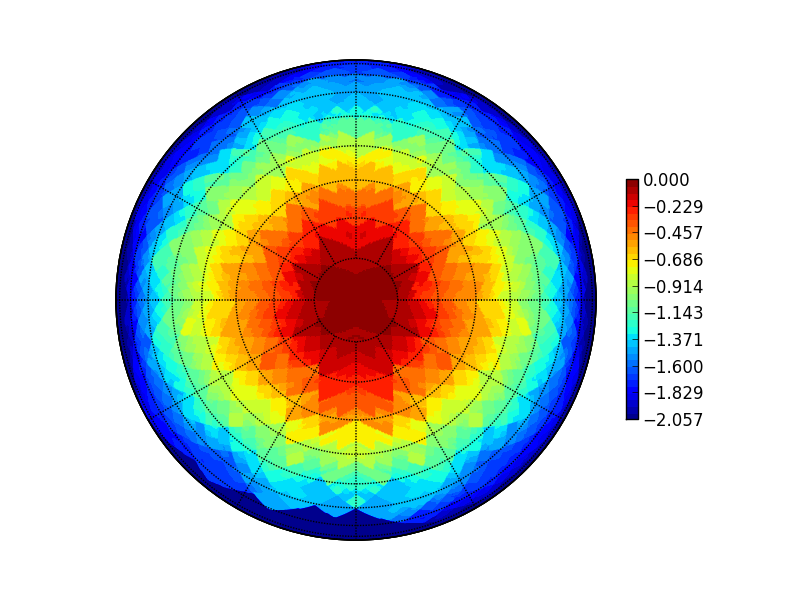
\includegraphics[width=.6\columnwidth]{plots/beam_raw.png}
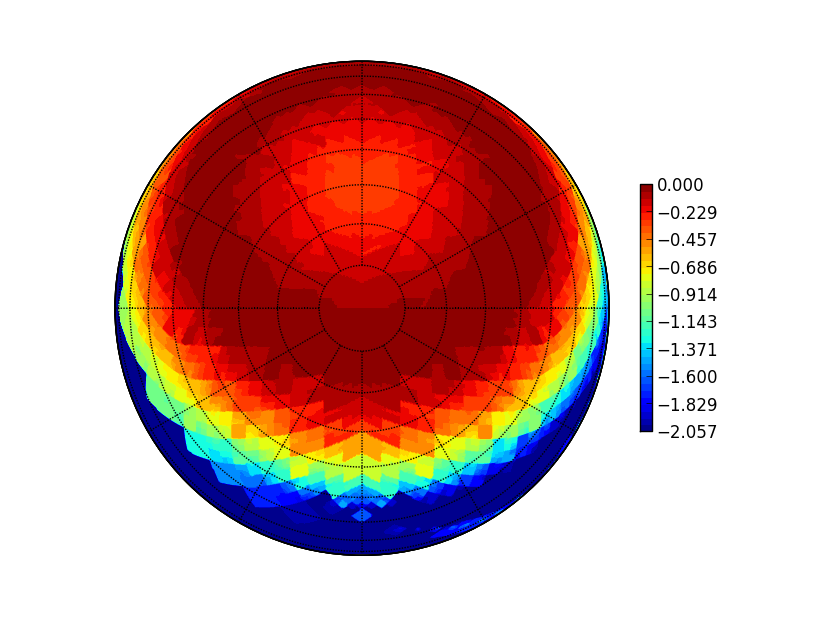
\includegraphics[width=.6\columnwidth]{plots/beam_wgt.png}
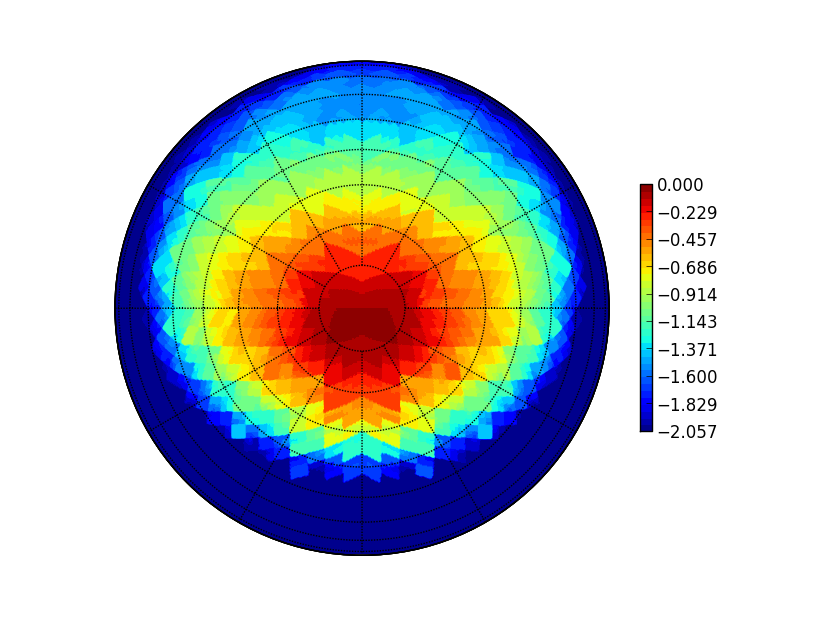
\includegraphics[width=.6\columnwidth]{plots/beam_fng.png}
\caption{
The effective primary beam response of a baseline, as determined from the simulations in \S\ref{sec:sim_pnt}.
Panels indicate reconstructions of PAPER's model beam response used in the simulation (left), the 
beam weighting that results from the application of a fringe-rate filter weighted to optimize SNR for
a 30-m baseline with PAPER's beam response (center), and the effective primary beam response of the
baseline after the application of the fringe-rate filter.
}\label{fig:}
\end{figure*}


\section{Matching Polarization Beams}
\label{sec:polbeams}

\section{Results and Discussion}
\label{sec:results}

\section{Conclusion}
\label{sec:conclusion}

\section{Acknowledgment}

% ---------------------------------------------------------------------
% ---------------------------------------------------------------------
% ---------------------------------------------------------------------

Similar geometric limits apply to the variation of visibilities in the time dimension.  As
described in Equation 7 of \citet{parsons_backer2009}, the rate of change of the geometric delay versus
time --- that is, delay-rate --- is given by
\begin{equation}
\frac{d\tau_g}{dt}=-\omega_\oplus\left(\frac{b_x}{c}\sin H + \frac{b_y}{c}\cos H\right)\cos\delta,
\end{equation}
where $\b=(b_x,b_y,b_z)$ is the baseline vector expressed in equatorial
coordinates, $\omega_\oplus$ is the angular frequency of the earth's rotation, and $H,\delta$ are the
hour-angle and declination of a point on the celestial sphere, respectively.  As a result, there exists a maximum
rate of change based on the length of a baseline projected to the $z=0$ equatorial plane.
For arrays not deployed near the poles, $|b_y|\gg|b_x|$ (i.e.,
they are oriented more along the east-west direction than radially from the polar axis),
and the maximum rate of change corresponds to $H=0$ and $\delta=0$, where we have
\begin{equation}
-\omega_\oplus\frac{|b_y|}{c}\le\frac{d\tau_g}{dt}\le\omega_\oplus\frac{|b_y|}{c}.
\end{equation}
For a maximum east-west baseline length in the PAPER array of 300m, $\omega_\oplus|b_y|/c$ is approximately
0.07 ns/s.  
To better elucidate the meaning of this bound, we take the Fourier transform 
along the time axis (see Equation 8 in \citealt{parsons_backer2009}) for a model visibility
consisting of a single point source located at the point of maximum delay-rate, which gives us
\begin{align}
\Vt(\nu,f)&\approx\At(\nu,f) * \tilde{S}(\nu) * \int{e^{2\pi i\omega_\oplus\frac{b_y\nu}{c}t}e^{-2\pi ift}dt}\nonumber\\
&\approx\At(\nu,f) * \tilde{S}(\nu) * \delta_{\rm D}(\frac{b_y}{c}\omega_\oplus \nu - f),
\end{align}
where $f$ is the fringe-rate of the 
source\footnote{Delay rate is equivalent to the frequency-integrated fringe rate.}, 
$\At(\nu,f)$ indicates the Fourier transform of the antenna response along the time direction,
and approximation is
indicated because we assume $|b_y|\gg|b_x|$, and because the Fourier transform must involve
a discrete length of time, during which our assumption that $\cos H\approx1$ breaks down at second order.
The delta function above gives rise to the expression for the maximum fringe rate in Equation \ref{eq:fringe_rate}.

This example of a source with a maximal fringe-rate serves to show that a 
filter may be applied in delay-rate domain, using the fact that the maximum
delay-rate is bounded by the maximum fringe rate within the band (i.e. evaluating Equation \ref{eq:fringe_rate}
at the maximum $\nu$ involved in the delay transform), to remove emission that exceeds the variation
dictated by array geometry for sources locked to the celestial sphere.  As in the delay filtering case, assuming
the geometric bounds on delay rate implicitly assumes that $\At$ and $\tilde{S}$ are compact in $f$, which
is to say that instrumental responses and celestial emission must be smooth in time; variable
emission from, e.g., fast-transients will be heavily suppressed by such delay-rate filters.
For PAPER, with a maximum baseline length of 300m and a maximum observing frequency of 200 MHz, 
the maximum delay-rate has a period of 68.5s.  As described in \S\ref{sec:fringe_rate_filtering}, at PAPER's
latitude, delay-rates range from -$f_{\rm max}/2$ to $f_{\rm max}$.  Filtering delay-rates to this
range corresponds in sensitivity to an effective integration time of 45.2 s.
An example of the bounds of a delay filter in DDR space is given
by the shaded magenta region in Figure \ref{fig:ddr_compression}.  As in the delay filtering case,
filtering along the delay-rate axis permits substantial down-sampling of the signal, which is
the basis for the reduction in data volume along the time axis.
We note that for the analysis
in \S\ref{sec:preprocessing}, we choose to use a slightly wider delay-rate filter to be conservative in
our first application of this technique, corresponding to an integration time of 43 seconds.

\section{On Calculating Beam Areas for Normalizing Power-Spectrum Measurements}
\label{app:beam_area}

We begin by examining the integrated volume, $\mathbb{V}$, used to normalize the 3D Fourier transform in
Equation 3 of P12a. We express this volume in observing coordinates as
\begin{equation}
    \mathbb{V} = \Omega B\cdot X^2Y,
\end{equation}
where $B$ is the bandwidth, $\Omega$ is the angular area, and $X,Y$ are redshift-dependent
scalars relating angle and frequency to spatial scales, respectively.
$\Omega$ arises from the bounds set by $A(l,m,\nu)$, the antenna power response, on the 
angular extent in the integral
\begin{align}
    \Vt^2(u,v,\eta)=&\left(\frac{2k_{\rm B}}{\lambda^2}\right)^2
        \left[\int{dl~dm~d\nu A(l,m,\nu)T(l,m,\nu)e^{-2\pi i(ul+vm+\eta\nu)}}\right]\times\nonumber\\
        &\left[\int{dl^\prime~dm^\prime~d\nu^\prime A^*(l^\prime,m^\prime,\nu^\prime)T^*(l^\prime,m^\prime,\nu^\prime)e^{2\pi i(ul^\prime+vm^\prime+\eta\nu^\prime)}}\right],
\end{align}
which is a slightly modified version of Equation 6 of P12a relating the delay-transformed visibility
$\Vt$, sampled at wavemodes $u,v$ (the Fourier complements of angular coordinates $l,m$) and $\eta$ (the Fourier
complement of spectral frequency $\nu$), to a temperature field $T$.
As shown in XXX, this reduces to
\begin{equation}
    {\tilde V}_{21}^2(u,v,\eta)\approx\left(\frac{2k_{\rm B}}{\lambda^2}\right)^2\frac{B}{X^2Y}
        \widehat P(\k)\int{dl~dm\left|A(l,m)\right|^2}.
\end{equation}

We compare this result with the relation between the delay-transformed visibility,
${\tilde V}$, to the three-dimensional power spectrum of reionization, $P_{21}(\k)$ 
(P12a):
\begin{equation}
    {\tilde V}_{21}^2(u,v,\eta)\approx\left(\frac{2k_{\rm B}}{\lambda^2}\right)^2\frac{\Omega\,B}{X^2Y} \widehat P_{21}(\k).
    \label{eq:v2_vs_pk}
\end{equation}
As this shows, the relevant beam area in Equation \ref{eq:v2_vs_pk} is the
power-square beam, $\Omega_{\rm PP}$, given by
\begin{equation}
\Omega_{\rm PP}\equiv\int{dl~dm\left|A(l,m)\right|^2}.
\label{eq:beam_squared}
\end{equation}
This contrasts with the standard metric for beam area --- the integrated
power beam --- which we will call $\Omega_{\rm P}$, and is given by
\begin{equation}
\Omega_{\rm P}\equiv\int{dl~dm A(l,m)},
\label{eq:beam_area}
\end{equation}
This beam area metric is used to convert visibility measurements from Jy units to mK,
but is incorrect for normalizing power spectra that relate to 
the two-point correlation function of a temperature field.

For equations that relate power-spectrum sensitivity to a system temperature
(e.g. Equations 15 and 16 in P12a)
\begin{equation}
\Omega^\prime\equiv\Omega_{\rm P}^2/\Omega_{\rm PP}
\end{equation}
should be used in lieu of $\Omega$, as
these equations pick up two factors of $\Omega_{\rm P}$ in the conversion from Jy$^2$ to mK$^2$, along with
the a factor of $\Omega_{\rm PP}$ in the denominator relating to the integrated volume.
For equations that relate a measured visibility (in units of brightness
temperature, e.g. Equation \ref{eq:pspec_cosmo}) to $\widehat P(\k)$, the factor of 
$\Omega_{\rm P}^2$ is already 
applied in the conversion from units of Jy to mK, 
and $\Omega$ corresponds to the remaining factor of $\Omega_{\rm PP}$. 

For PAPER, $\Omega_{\rm P}\approx0.72$ sr, while $\Omega_{\rm PP}$ is 0.31 sr.  Following the definition
above, $\Omega^\prime\approx1.69$.  These beam areas are calculated numerically from
a beam model, but typically, $\Omega^\prime$ is about a factor of two larger than $\Omega_{\rm P}$.

%\clearpage
\bibliographystyle{apj}
\bibliography{biblio}

\end{document}

